% Seccion de Diseno y construccion 

%%\chapter{Integración de componentes}
%\section{Diseño y Construcci\'on}

%El primer paso ha sido la construcci\'on de la parte física del robot. Para tal fin se procedió a la elección del diseño y ensamblaje de las piezas. En la sección \ref{subsection:diseno} se describe cada uno de los componentes utilizados para armar el robot, y luego, en la secci\'on \ref{subsection:construccion} se explica cómo se integraron esas piezas para obtener un humanoide adaptado a los objetivos de este proyecto.
\section{Partes del robot}\label{sec:diseno}

%\label{subsection:componentes}
%\subsection*{Componentes de hardware}
A continuación se presenta una descripción de los elementos que han sido seleccionados para la construcción del robot humanoide. 

Las opciones que se han considerado para la construcci\'on del cuerpo de Junny han sido: 
\begin{itemize}
  \item Uso de piezas de \gls{LEGO}.
  \item Construcci\'on y dise\~no mec\'anico desde cero.
  \item Uso de las piezas del kit Bioloid \cite{robotics}.
\end{itemize}

Estas opciones corresponden a los recursos disponibles. Tanto la construci\'on con piezas de \gls{LEGO} como la opci\'on de realizarlo desde cero implicaba más tiempo del que se disponía, adem\'as que realizarlo en su totalidad con dise\~no mec\'anico y electr\'onico implicaba conocimientos m\'as avanzados en el \'area de mecatr\'onica que no eran el objetivo del proyecto. Por lo tanto se escogi\'o su construcci\'on con el kit Bioloid como la opci\'on m\'as factible para el cumplimiento de los objetivos. 

El kit Bioloid es un kit de robótica con piezas prefabricadas que permite armar diferentes tipos de robot pero principalmente humanoides. Su empaque se puede observar en la figura ~\ref{fig:kit}. El fabricante, Robotics \cite{robotics}, incluye un manual  con varios modelos de robots con instrucciones de ensamblaje. Provee una tarjeta controladora, CM-510 \cite{cm510}, a la que se conectan los motores Dynamixel y algunos sensores que se programan a través de la interfaz de ‘RoboPlus’ \cite{robotics}.

\begin{figure}[hbtp]
\centering
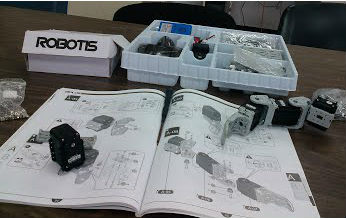
\includegraphics[scale=0.5]{imagenes/kitAfuera.jpg}
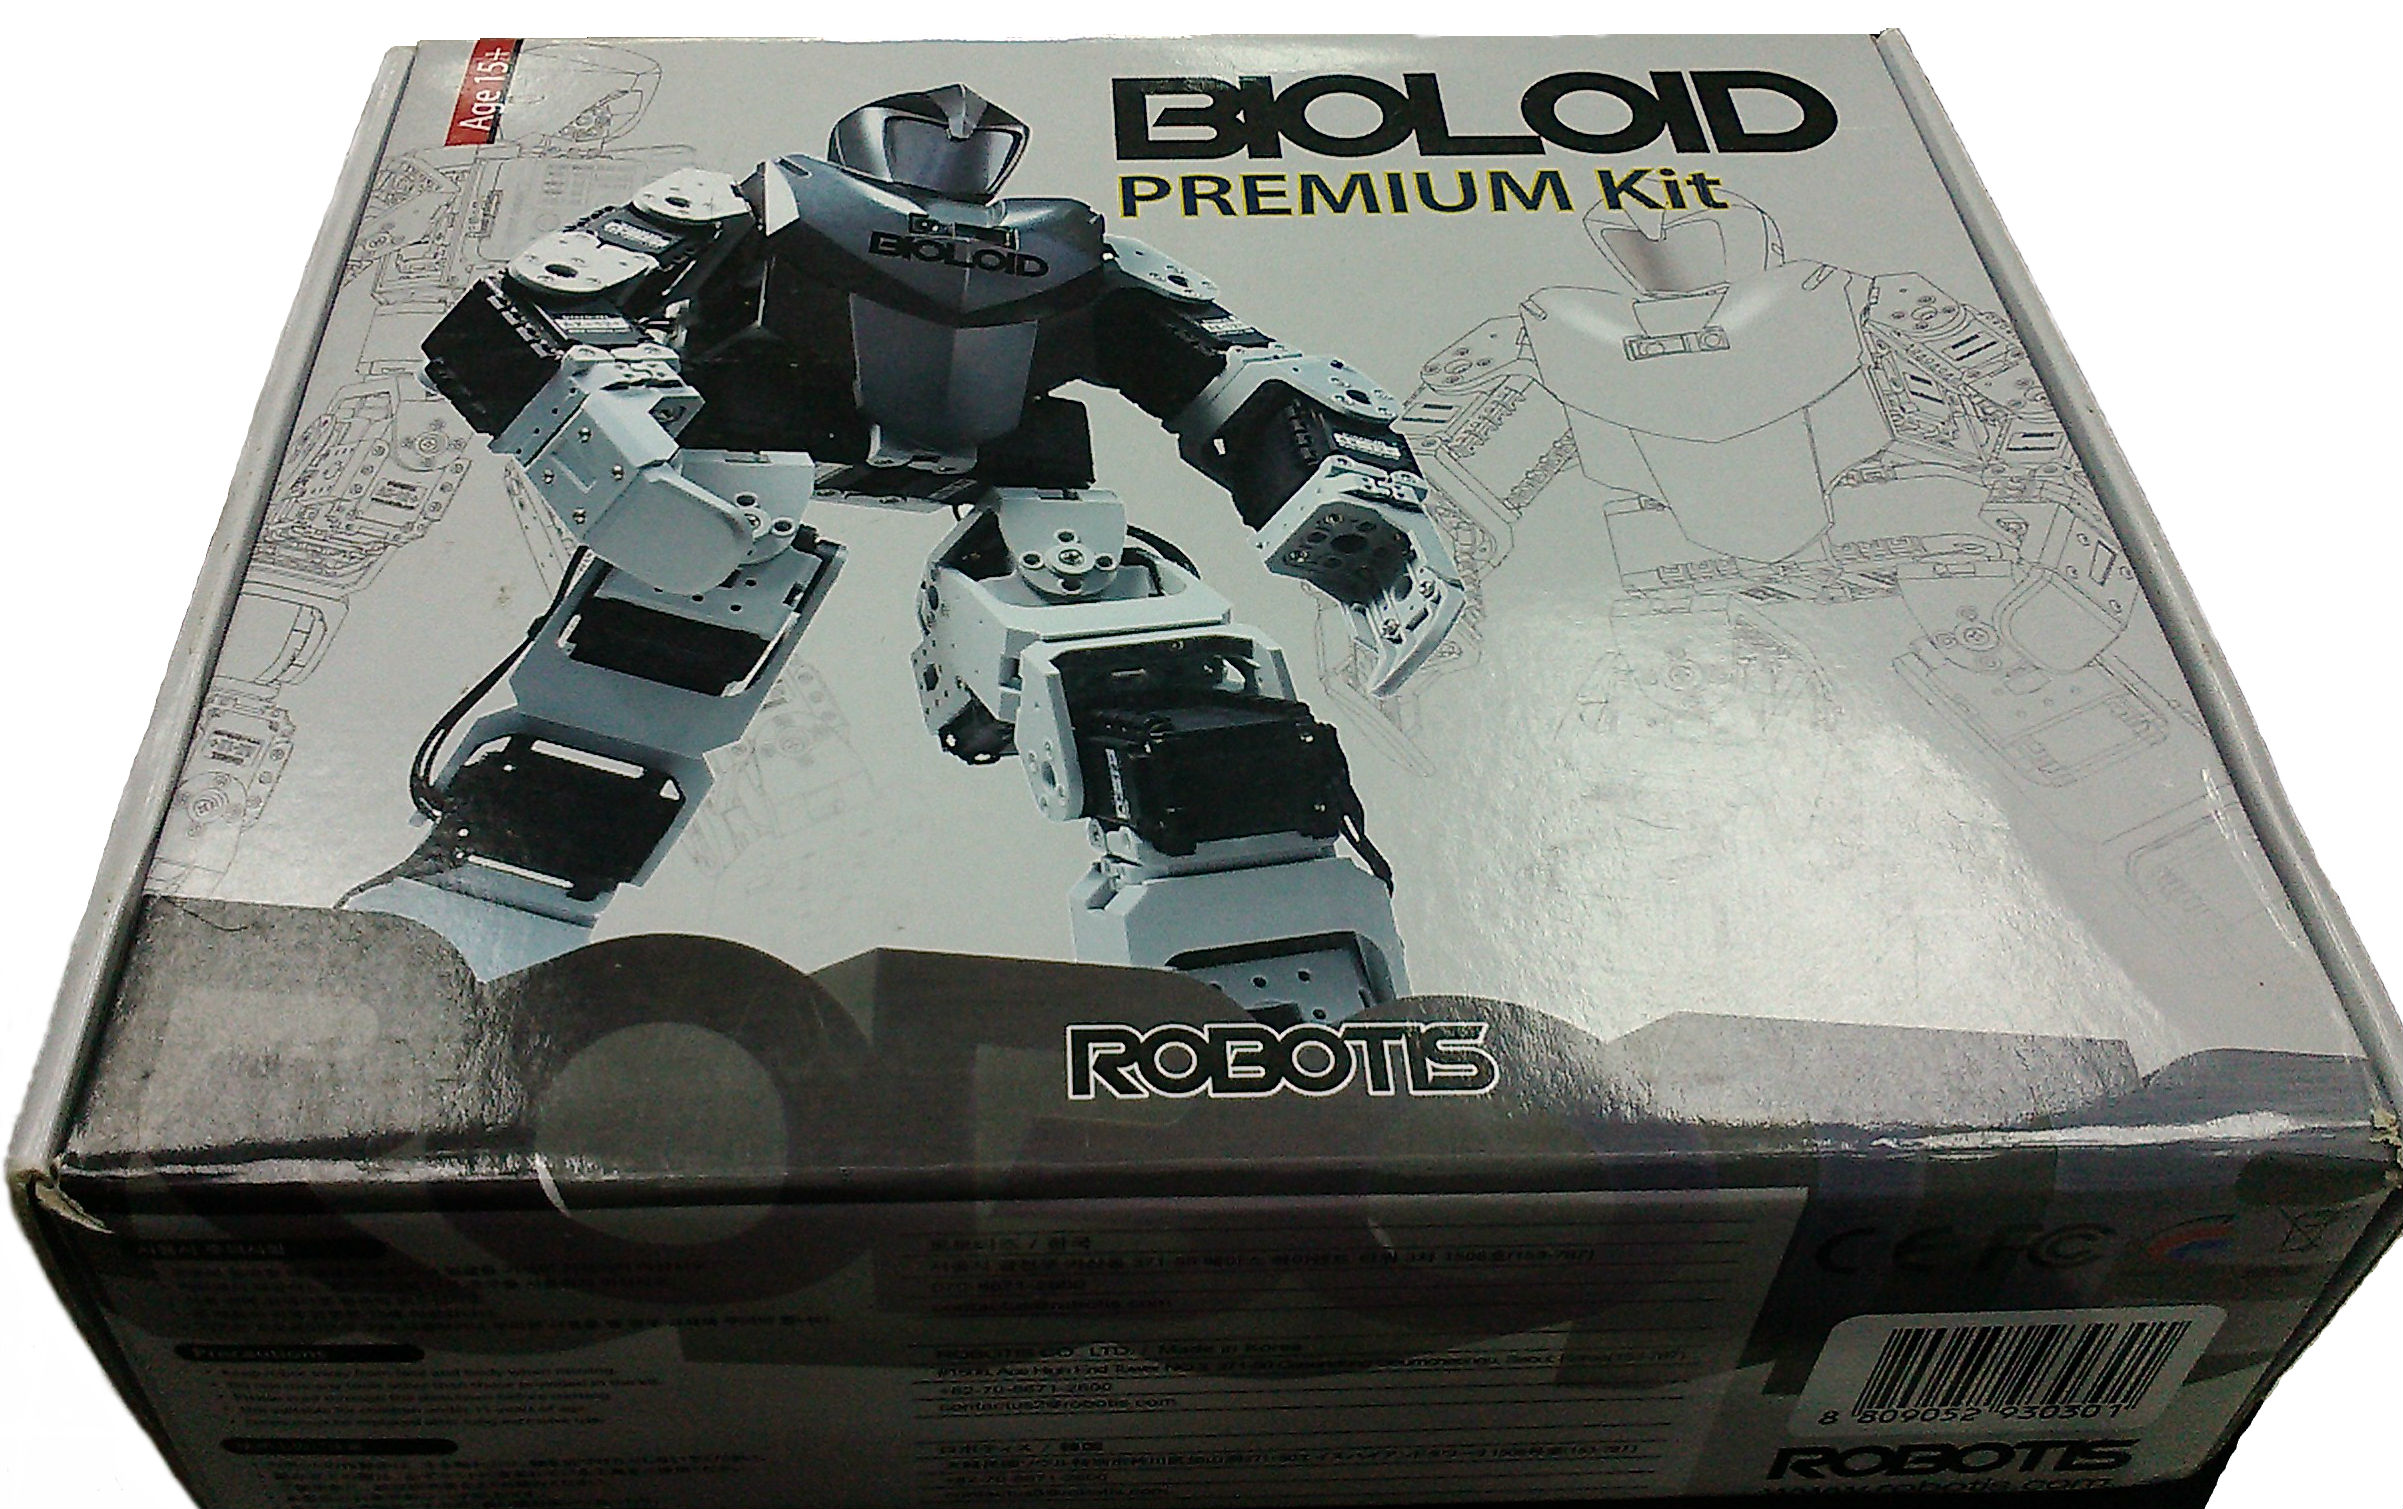
\includegraphics[scale=0.07]{imagenes/cajaKit.jpg}
\caption{Bioloid Premium Kit}
\label{fig:kit}
\end{figure}

Se decidi\'o sustituir la tarjeta controladora CM-510 por la tarjeta controladora de software libre Arbotix. La utilización de la tarjeta Arbotix permite una mayor flexibilidad en el control de motores y la incorporación de una variedad de sensores no soportados por la tarjeta CM-510.
Además, la tarjeta Arbotix posee mayor soporte y amplitud en la comunicación entre distintos dispositivos, permite el control avanzado de algunos tipos de servos Dynamixel y robots basados en Bioloid. Incorpora un microcontrolador \gls{AVR}, radio inalámbrica \gls{XBEE}, conductores de motor dual, y cabeceras de estilo servo de 3 pines para entrada/salida digital y analógica \cite{arbotix}.

Los Motores Dynamixel Ax-12+ son actuadores inteligentes y modulares que incorporan un reductor de engranajes, un motor DC de precisión y un circuito de control con funcionalidad de red lo cual permite formar series o cadenas de motores como se muestra en la figura ~\ref{MotorBateria}. Estos motores están incorporados en el kit Bioloid al igual que la batería de polímero de litio (LiPo), fuente de poder para motores y componentes electr\'onicos. La batería empleada es de 11.1 Voltios y 1 Amperio. \cite{bateria}


%\begin{figure}[hbtp]
%\centering
%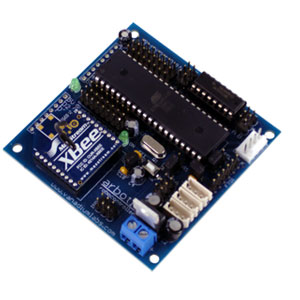
\includegraphics[scale=0.5]{imagenes/ARBOTIX.JPG}
%\caption{Tarjeta controladora ArbotiX}
%\end{figure}

\begin{figure}[hbtp]
\centering
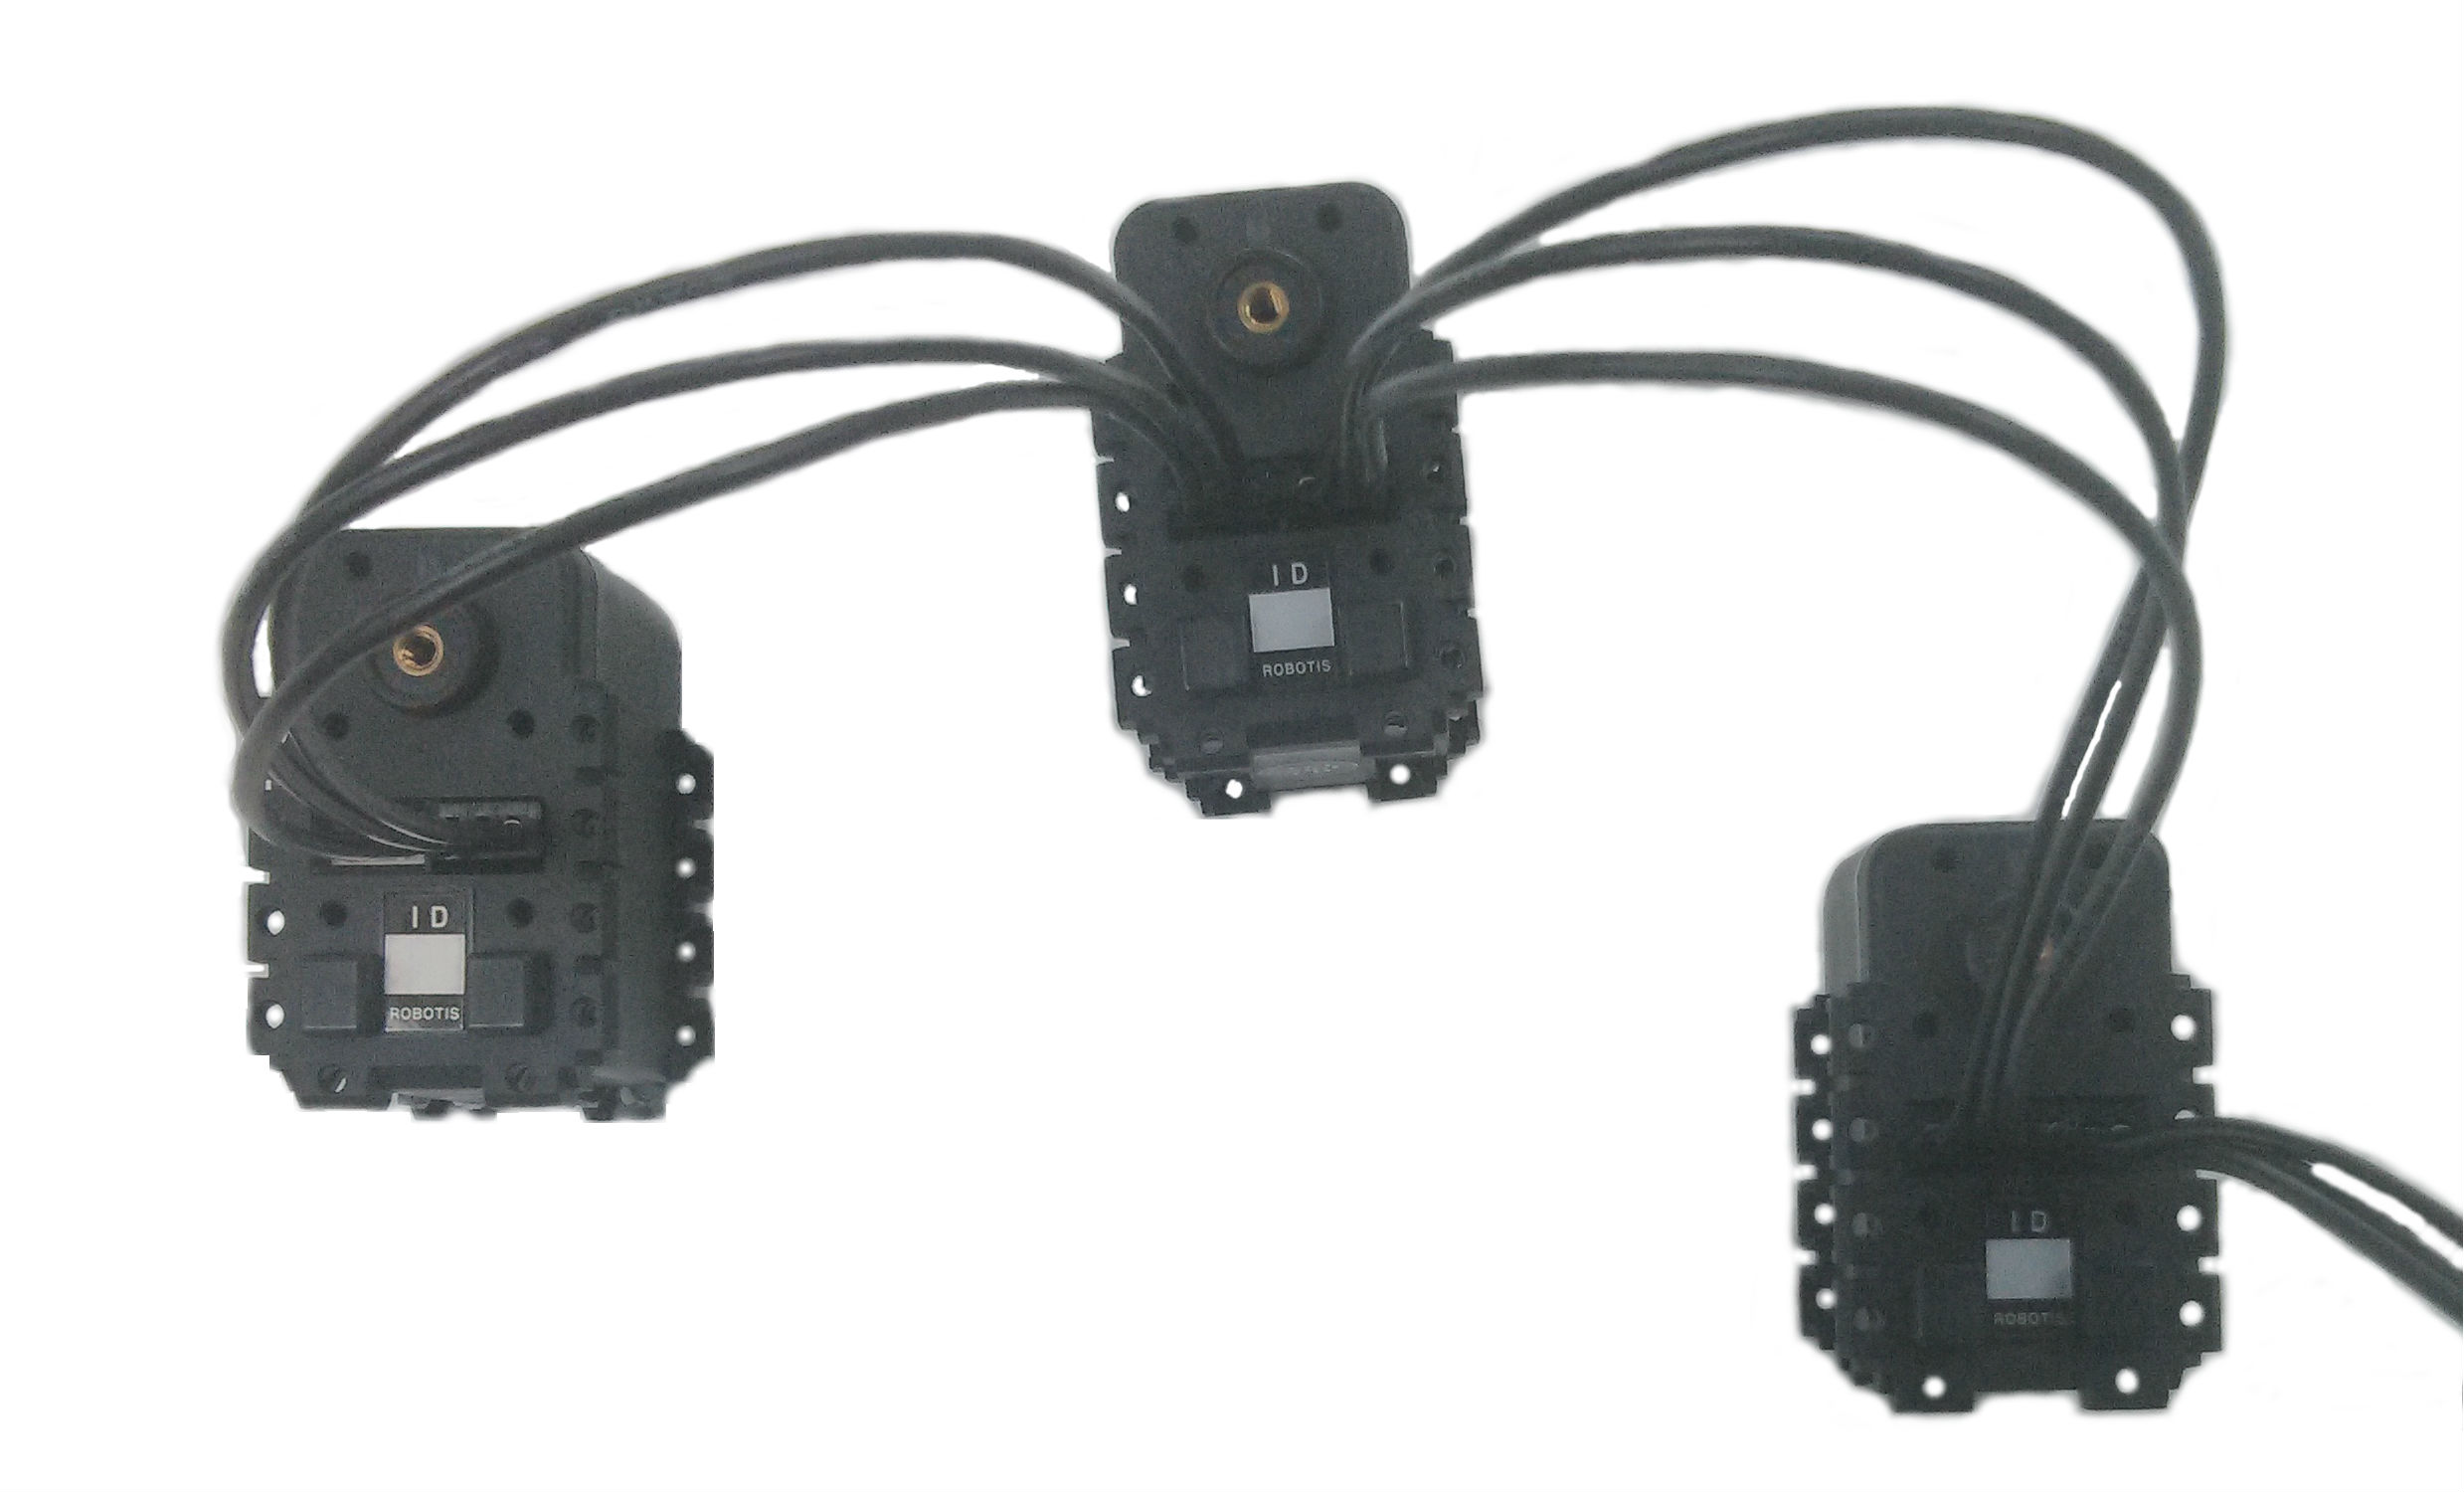
\includegraphics[scale=0.08]{imagenes/3Dynamixel.jpg}
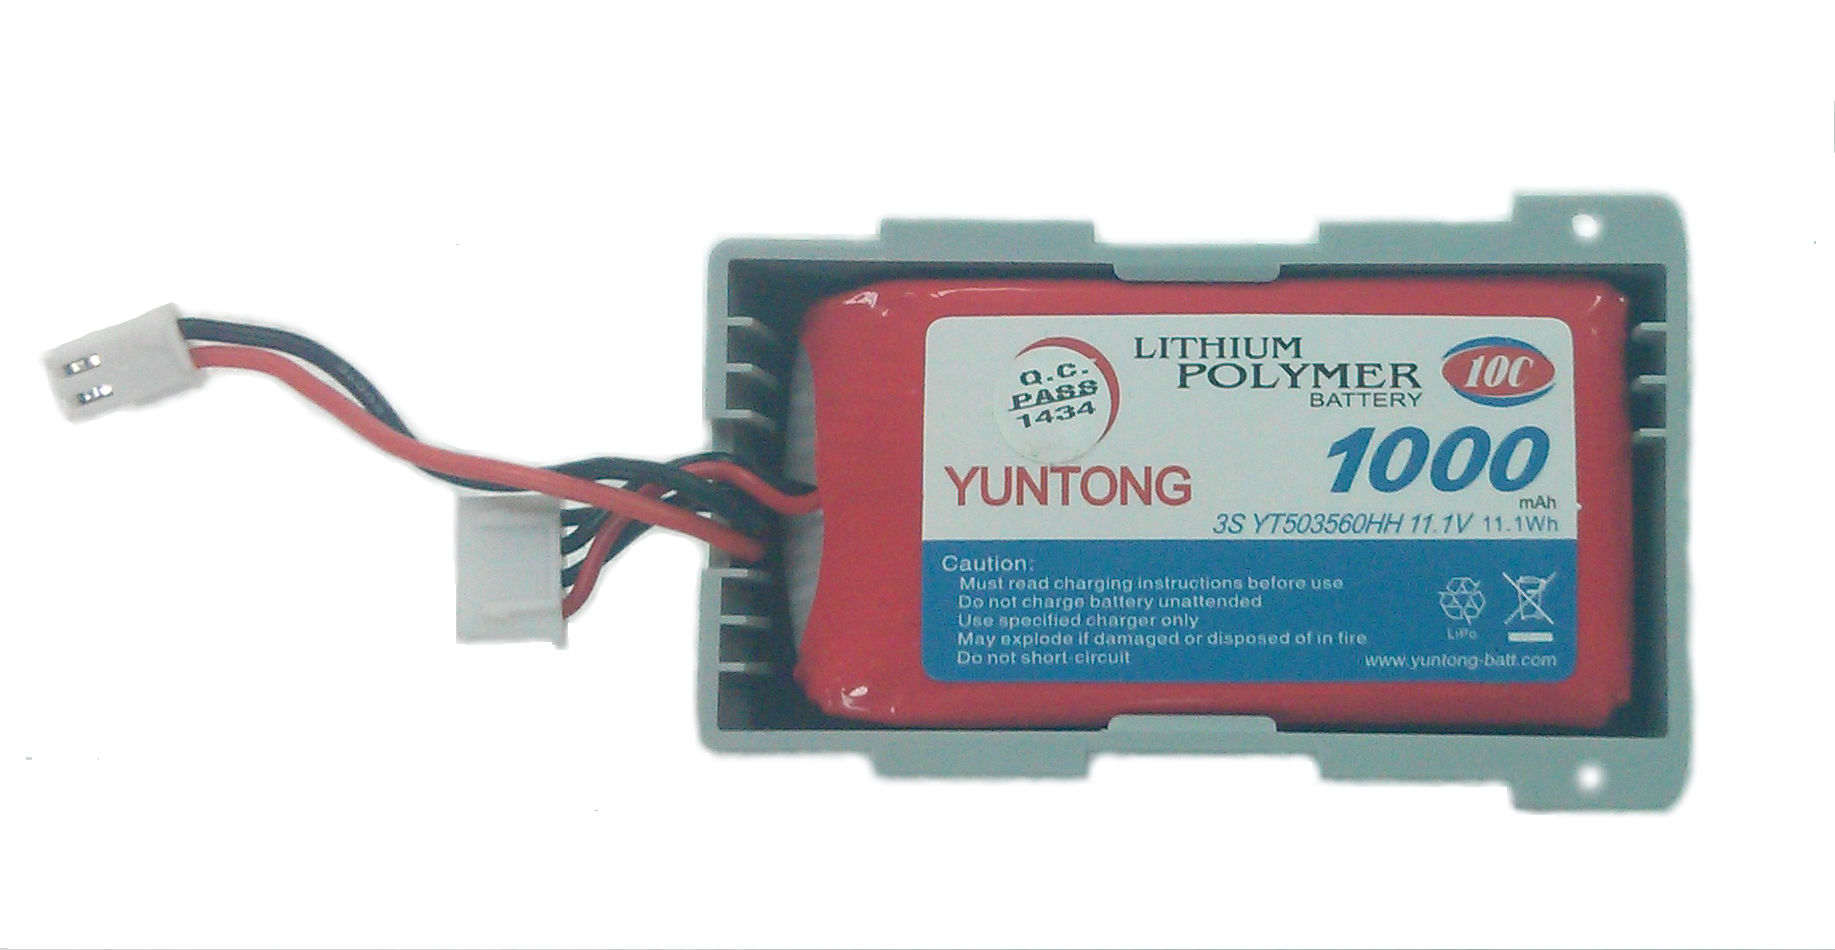
\includegraphics[scale=0.08]{imagenes/bateriaLipo.jpg}
\caption{A la izquierda, 3 motores Dynamixel conectados en serie. A la derecha, batería LiPo}
\label{MotorBateria}
\end{figure}

%\begin{figure}[hbtp]
%\end{figure}

Para la detecci\'on de ca\'idas se ha seleccionado un giroscopio (Robotics Gyro) que mide la velocidad angular que genera los movimientos del robot, este se encuentra diseñado para verificar el balance del robot y ser usado para otras aplicaciones de movimiento \cite{gyro}. También se encuentra incluido en el kit Bioloid. En la figura ~\ref{fig:gyroYextensor} se puede observar su estructura. Existen otros sensores de inercia que se enfocan en realizar la tarea de balance y orientaci\'on del robot como el aceler\'ometro, sin embargo estos no se encontraban disponibles en el laboratorio.

\begin{figure}[hbtp]
\centering
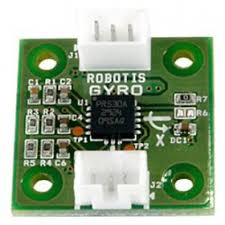
\includegraphics[scale=0.35]{imagenes/gyro.jpg}
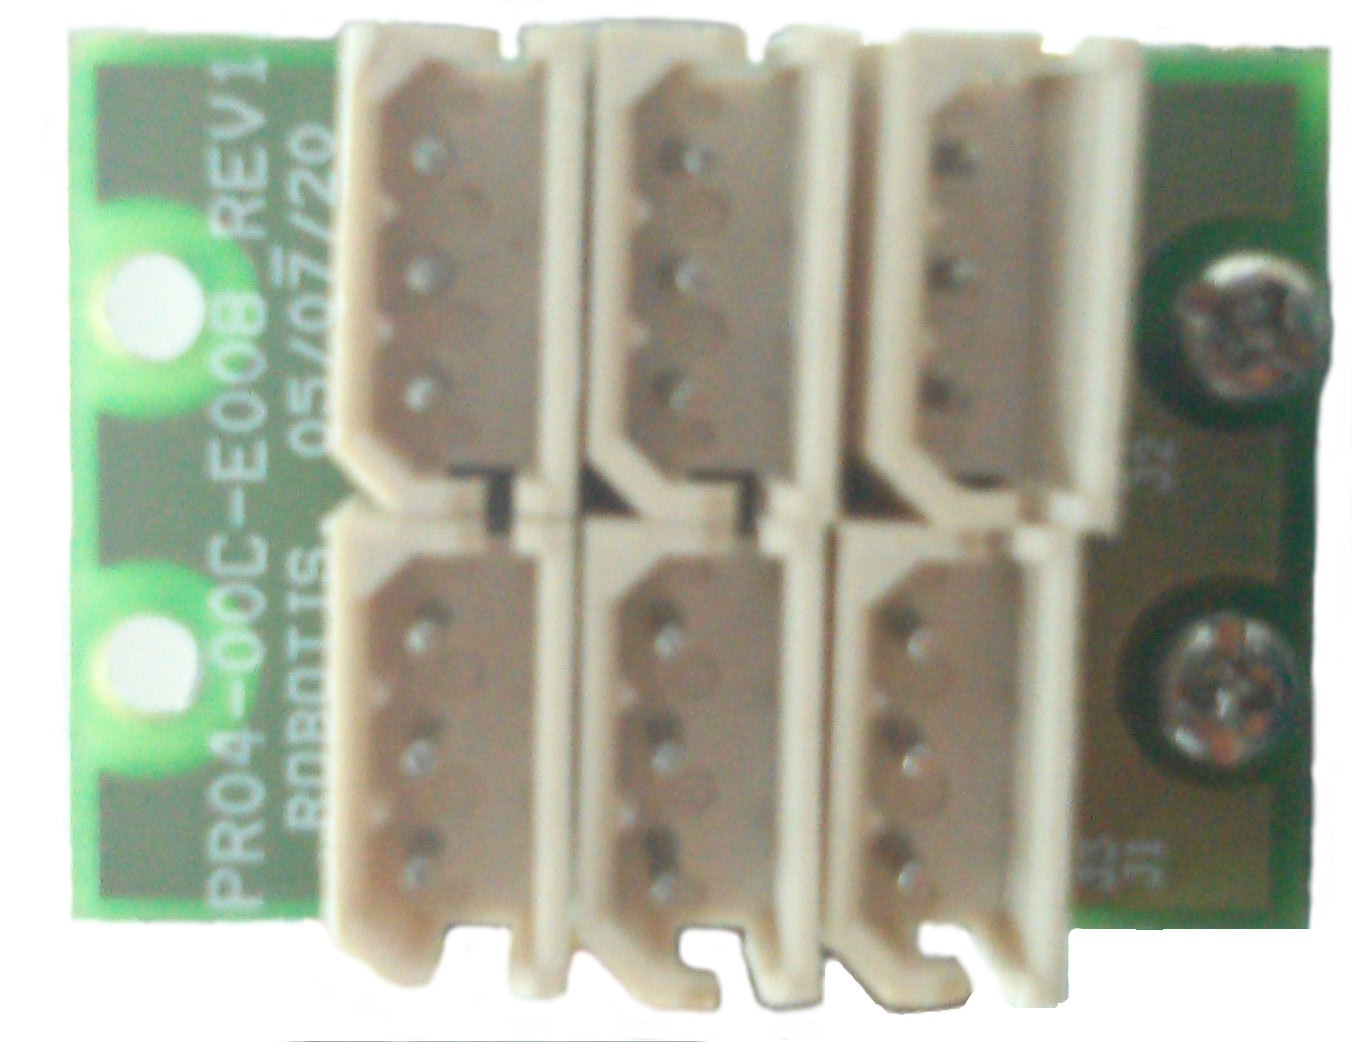
\includegraphics[scale=0.08]{imagenes/extensor.jpg}
\caption{A la izquierda, sensor Gyro. A la derecha, extensor de puertos Bioloid}
\label{fig:gyroYextensor}
\end{figure}

Ha sido necesario incluir un extensor de puertos Bioloid que permitiera conectar un mayor n\'umero de motores Dynamixel, este se muestra en la figura ~\ref{fig:gyroYextensor} \cite{hub}. En la siguiente secci\'on se explica como han sido conectados los motores y el motivo para incluir el expansor. 
%fue necesario para una mejor movilidad del robot pues se dividi\'o su cuerpo en cuatro extreminades por lo tanto cuatro series de motores distintas y el expansor permite aumentar el número de cadenas de servos conectados a la tarjeta


Para agregar mayor capacidad de procesamiento, con la finalidad de poder captar y procesar imágenes, se incorpor\'o el mini computador Raspberry Pi, de aproximadamente 10 cm de largo, 5 cm de ancho y 2 cm de alto, a la que se puede conectar un módulo de cámara especialmente diseñado para él. Puede ser utilizado en proyectos de electrónica y para varias de las tareas que un computador de escritorio puede hacer, como procesamiento de hojas de cálculo y de texto, ejecutar juegos, entre otras \cite{raspberry}. Su estructura se puede ver en la figura ~\ref{fig:RaspYcamara}. La Raspberry Pi cuenta con un procesador gráfico que permite aligerar la carga del procesador central \cite{elLinux}. Para las funciones correspondientes a la Rasberry Pi, en el proyecto tambi\'en era factible la utilizaci\'on de un tel\'efono celular avanzado, sin embargo esta opci\'on fue decartada pues agrega un peso importante a la estructura del robot, dificultad para añadirle grados de libertad a su cámara y un costo superior al de la Raspberry.  

Para lograr el objetivo de detecci\'on de la pelota y orientaci\'on al arco existía la posibilidad de añadir un sensor de br\'ujula y un sensor de proximidad. Sin embargo la ulitizaci\'on de una c\'amara para esta tarea representaba mayores ventajas. La cámara posee un mayor rango de percerpción, aumentando las posibilidades de encontrar la pelota o arco en menor cantidad de tiempo que con los sensores. Adem\'as, la incorporación de la Raspberry Pi  \cite{raspberry} y su cámara permite la posibilidad de ampliar las habilidades y tareas que podr\'ia realizar Junny. La c\'amara puede captar im\'agenes y grabar vídeos de alta definición. Tiene 5 megapíxeles de foco fijo que soporta los modos de vídeo de 1080x30, 720x60 y \gls{VGA}90. Puede ser manejada con las librerías \gls{MMAL}, \gls{V4L} u otras librerías de terceros como la de Python \cite{raspberrycam}

%(http://www.raspberrypi.org/products/camera-module/)
% Se conecta a la Raspberry Pi con un cable de cinta plana de 15 cm en el puerto CSI.

\begin{figure}[hbtp]
\centering
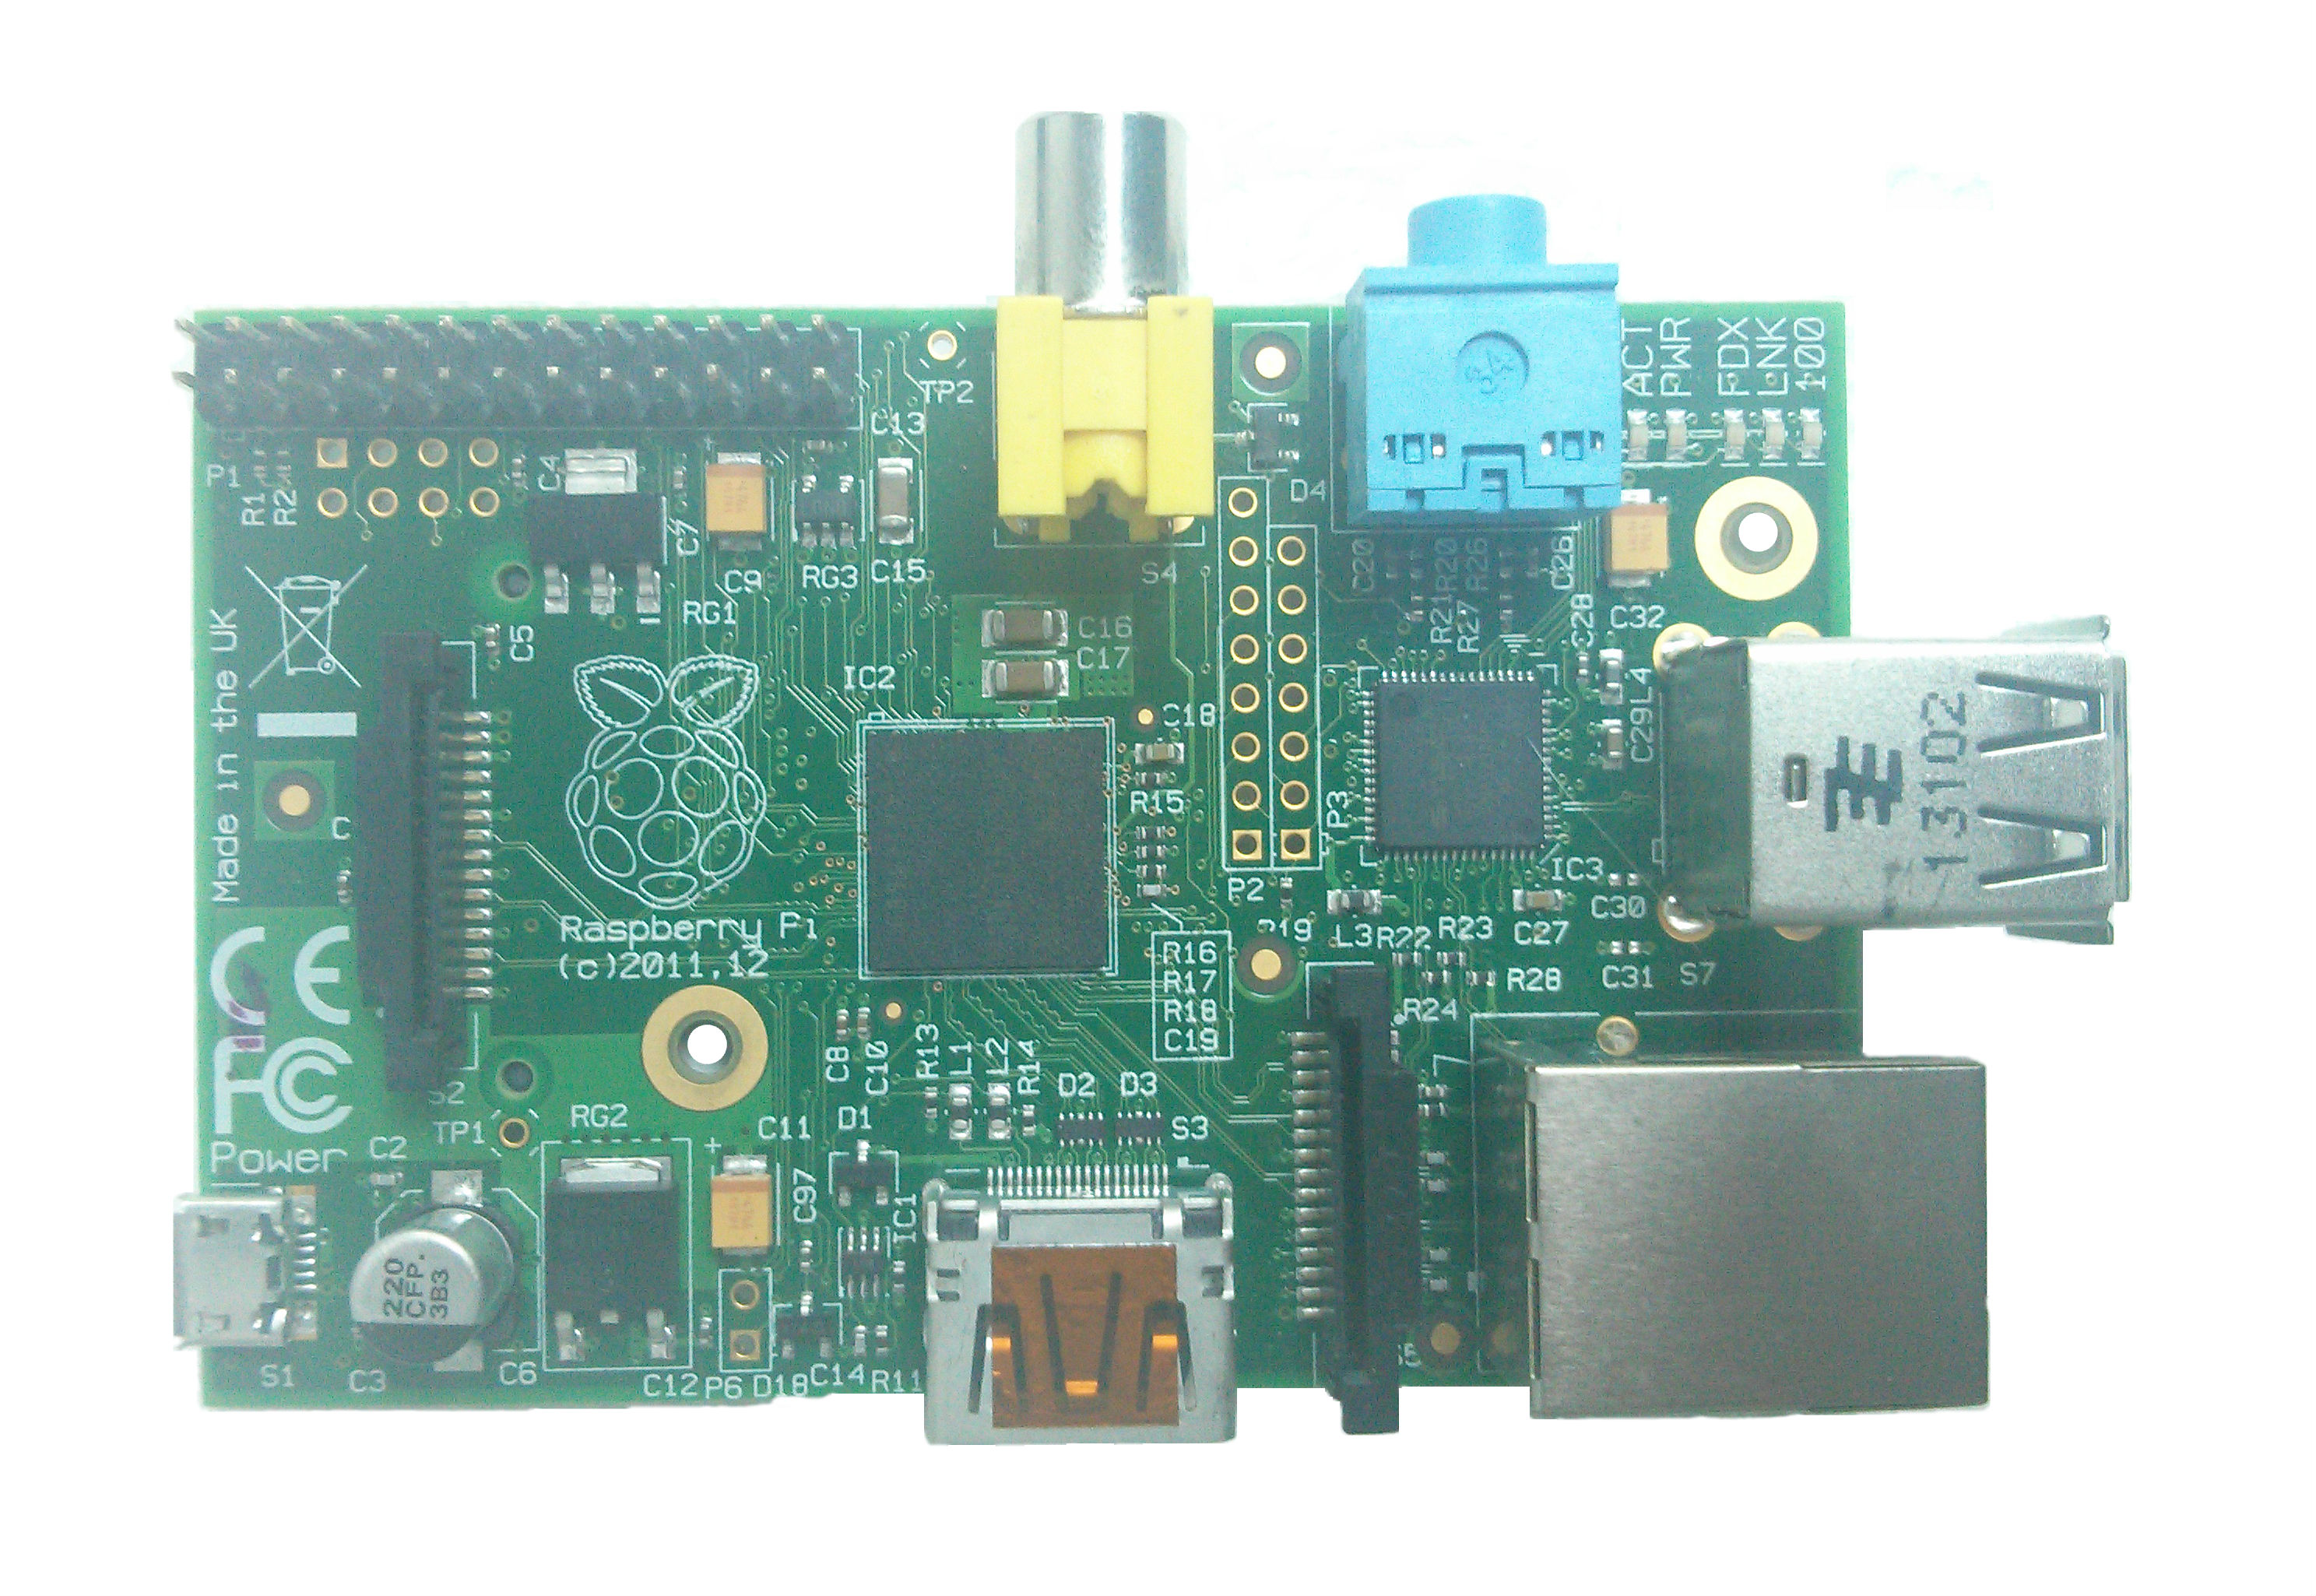
\includegraphics[scale=0.06]{imagenes/RaspberryPi.jpg}
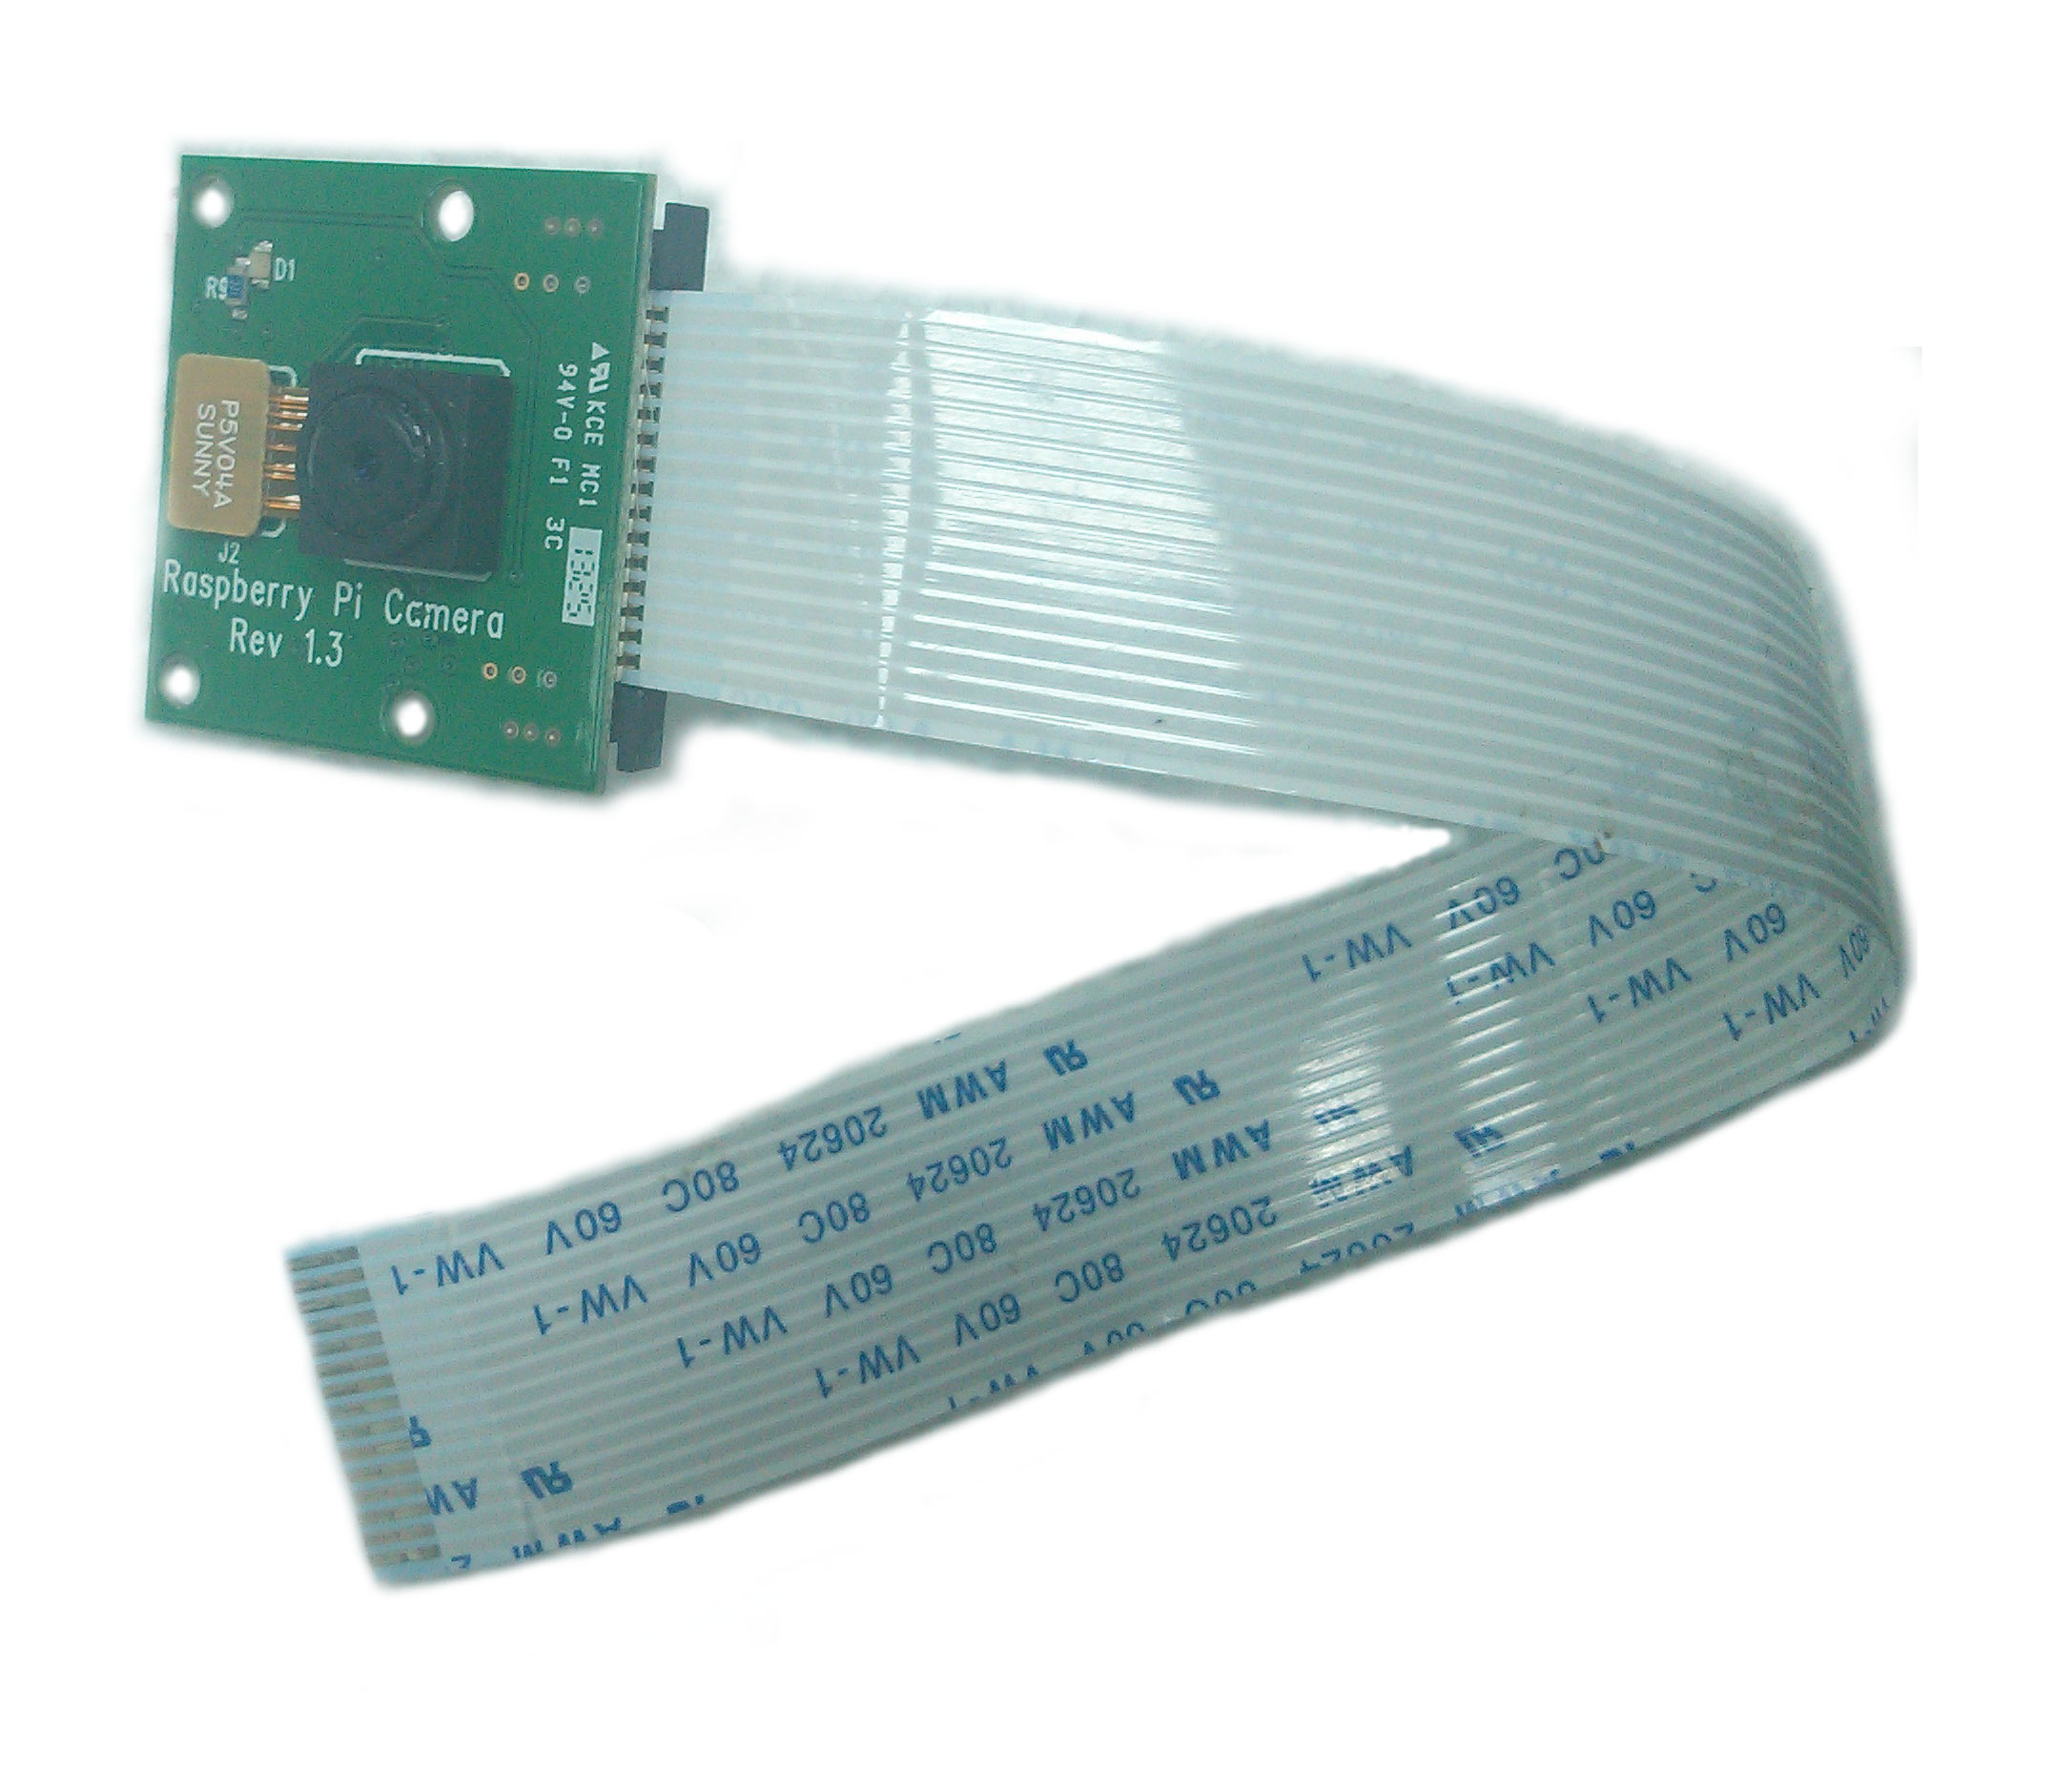
\includegraphics[scale=0.06]{imagenes/CamRasp.jpg}
\caption{Tarjeta Raspberry Pi y su módulo de cámara a la derecha}
\label{fig:RaspYcamara}
\end{figure}

Para poder establecer la comunicación entre la Arbotix y la Raspberry Pi, se añadió el chip FTDI (Future Technology Devices International) \cite{ftdi}. Es una tarjeta controladora  (se puede observar en la figura ~\ref{fig:ftdi}) que ofrece el servicio de conversión de  datos de \gls{USB} a \gls{UART}, por lo cual permite la comunicación entre diferentes dispositivos \cite{ftdi}. Fue elegida en lugar de la radio inálambrica \gls{XBEE}, pues la Raspeberry Pi y la Arbotix estan f\'isicamente cerca lo cual permite usar cableado directo, y usar los \gls{XBEE} implicaba un mayor costo para el proyecto.

Para añadir grados de libertad a la c\'amara se utilizaron como base dos micro servomotores anal\'ogicos TG9e \cite{microservo}. La capacidad de torque de estos motores alcanza los 1.50 kg-cm . Permiten ser controlados en posición en un rango de 180$^{\circ}$. Ver figura ~\ref{fig:Servo}.   

\begin{figure}[hbtp]
\centering
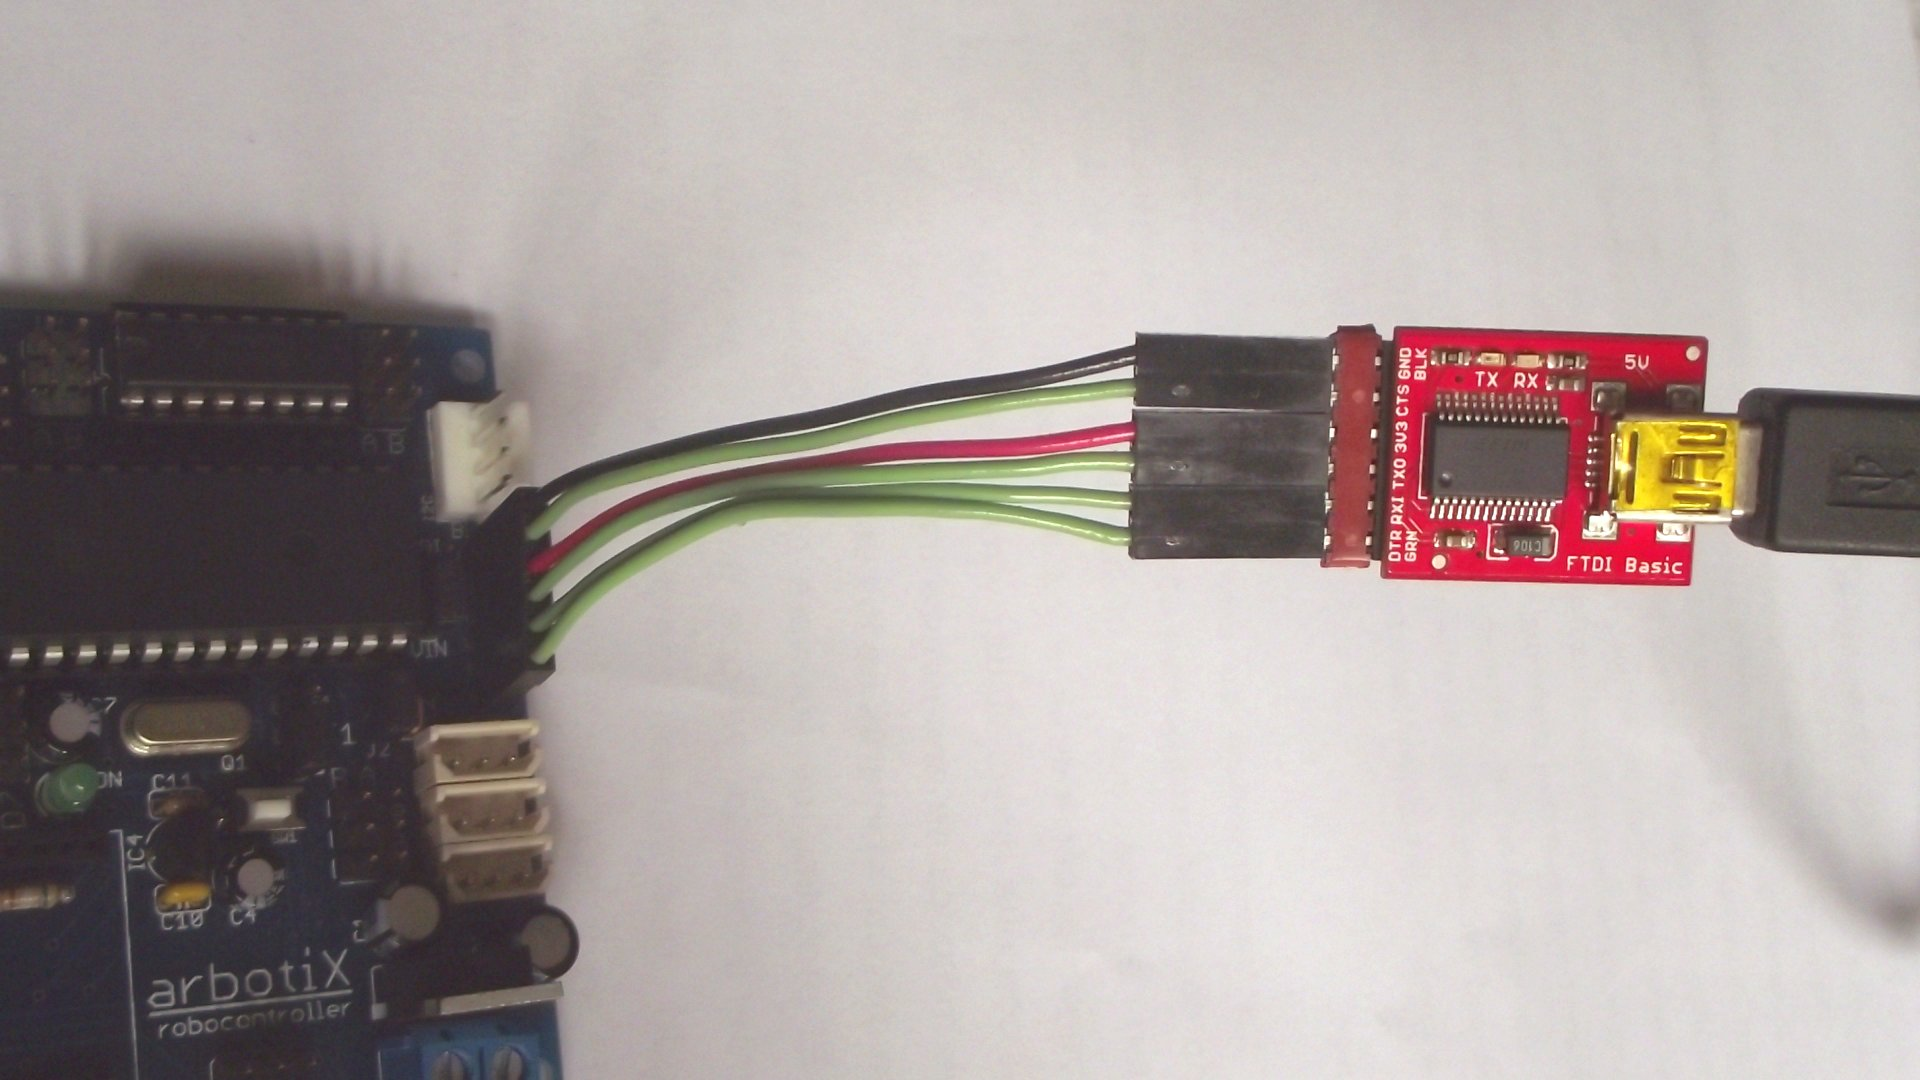
\includegraphics[scale=0.06]{imagenes/DSCF1162.jpg}
\caption{Chip FTDI conectado a la tarjeta Arbotix}
\label{fig:ftdi}
\centering
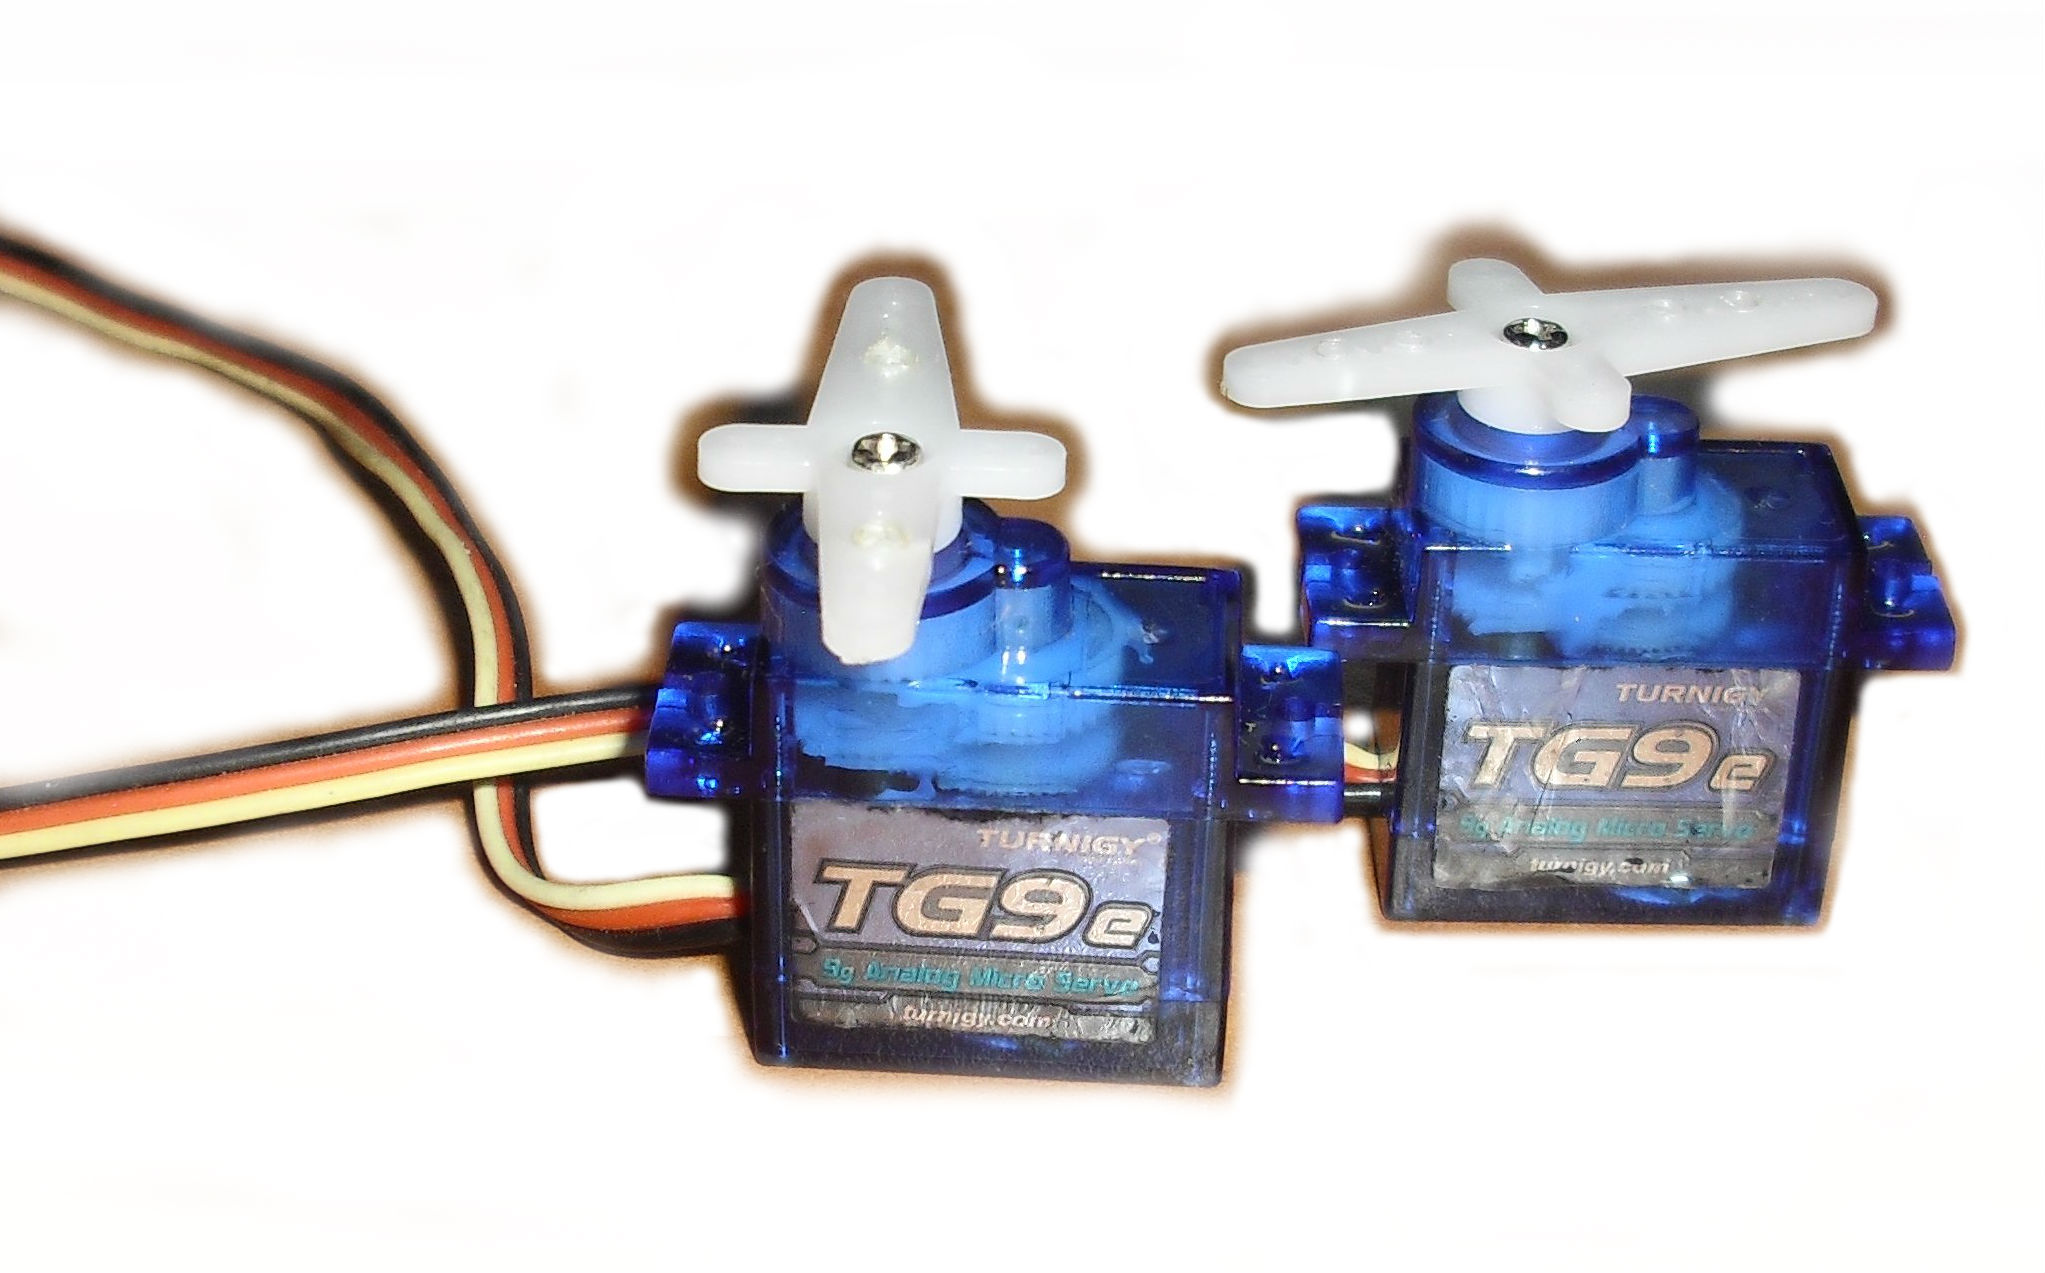
\includegraphics[scale=0.09]{imagenes/servosTg9B.jpg}
\caption{Micro Servomotores analógicos TG9e}
\label{fig:Servo}
\end{figure}

Debido a que no todos los componentes poseen las mismas exigencias con respecto a voltaje y amperaje, se realizó un regulador (ver figura ~\ref{fig:circuito}) con una salida de 5 voltios para la tarjeta Raspberry Pi y dos micro servomotores, y otra salida de 11.1 V para la tarjeta Arbotix que a su vez alimenta a los componentes conectados en ella (motores Dynamixel y Giroscopio). Si bien la tarjeta Arbotix posee un regulador interno de cinco voltios la opción de conectar todo a la salida de 5 V del regulador no era posible, dado que los motores Dynamixel requieren alimentación de 11 voltios.

\begin{figure}[hbtp]
\centering
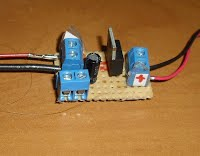
\includegraphics[scale=0.5]{imagenes/circuito.jpg}
\caption{Circuito con entrada de 11.1 V. Una salida de 5 V para los micro servomotores anal\'ogicos y tarjeta Raspberry Pi. Otra salida de 11.1 V para alimentar la controladora Arbotix.}
\label{fig:circuito}
\end{figure}

%\begin{figure}[hbtp]
%\centering
%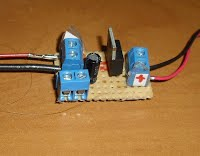
\includegraphics[scale=0.7]{imagenes/circuito.jpg}
%\caption{Lipo}
%\end{figure}

\section{Ensamblaje}\label{subsection:construccion}

Como se mencionó anteriormente para la construcción del robot se utilizó el kit de piezas Bioloid Premium de marca Robotis el cual incluye motores Dynamixel Ax-12+, una tarjeta controladora CM-510, un sensor Gyro, un manual \cite{manualRobot}, entre otros elementos. El manual incluye las instrucciones de como armar los modelos A, B y C de humanoide, el utilizado en este proyecto es el tipo B, haciendo uso de 16 motores. En las figuras ~\ref{fig:frontal} y ~\ref{fig:trasera1}  se puede observar la estructura del robot que aparece en el manual del kit. La elecc\'ion de este modelo se debi\'o a que los motores como recuersos eran escasos y a pesar de que el modelo A posee un grado más de libertad que los otros modelos (incluye tanto los de B como los de C) utiliza dos motores más que los otros dos modelos. El modelo B posee un grado de libertad de interés a la hora de girar del robot, que el modelo C no posee, por ello se eligi\'o este.

\begin{figure}[hbtp]
\centering
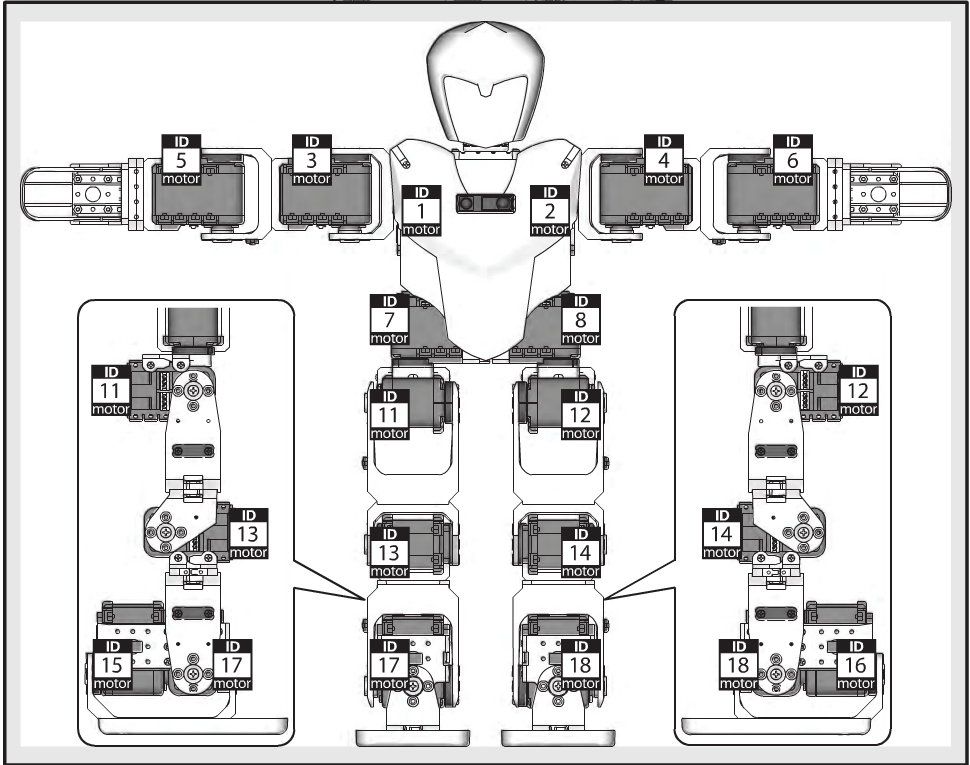
\includegraphics[scale=0.3]{imagenes/Robot.png}
\caption{Vista frontal del robot, tipo B. Se puede apreciar la identificación ‘ID’ de cada motor Dynamixel Ax-12+. Nota: los motores 9 y 10 no se utilizan. Imagen tomada sin autorizaci\'on de \cite{manualRobot}}.

\label{fig:frontal}
\end{figure}

\begin{figure}[hbtp]
\centering
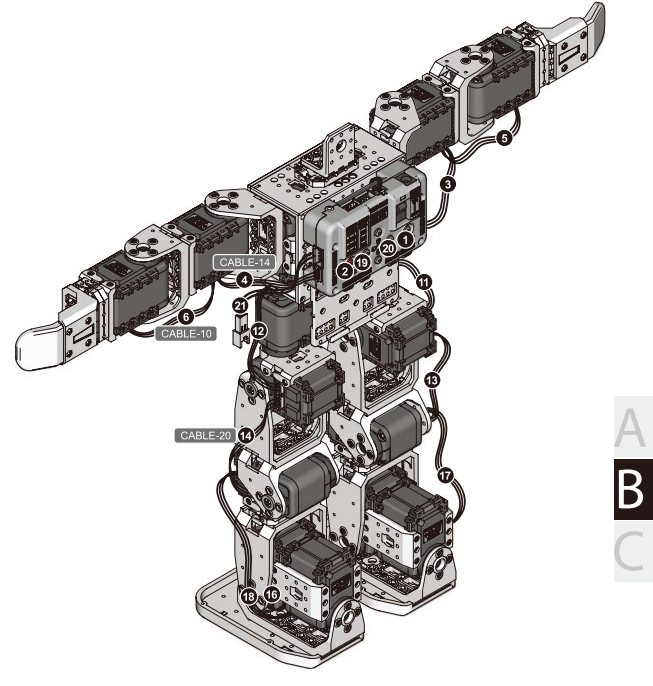
\includegraphics[scale=0.3]{imagenes/RobotTrasero.png}
\caption{Vista trasera del robot con la tarjeta CM-510, Imagen tomada sin autorizaci\'on de \cite{manualRobot}.}
\label{fig:trasera1}
\end{figure}


En la figura ~\ref{fig:trasera2} se puede observar la estructura del robot con la Arbotix incorporada. En la parte interna del tronco del robot se sitúa el sensor Gyro.

\begin{figure}[hbtp]
\centering
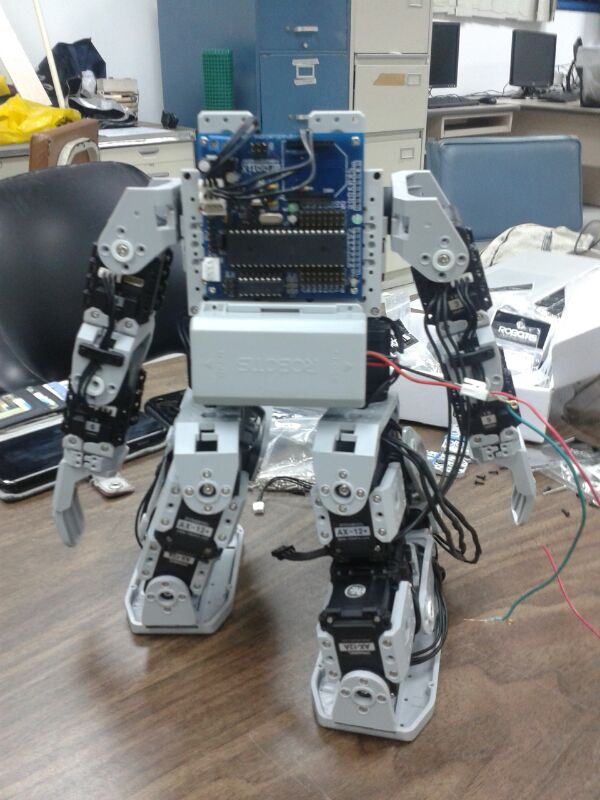
\includegraphics[scale=0.2]{imagenes/traseroDeJunny.jpg}
\caption{Vista posterior del robot, con la tarjeta Arbotix integrada (tarjeta azul) y la bateria LiPo }
\label{fig:trasera2}
\end{figure}

Para el movimiento de la cámara se ha incorporado dos micro servomotores TG9e ya que estos poseen un tama\~no reducido perfecto para acoplarlo en la estructura al igual que su peso, uno para el movimiento horizontal y otro para el vertical. La conexión de uno de estos motores se ilustra en la figura ~\ref{fig:arbotixConectados}, en donde se puede observar que se encuentra conectado al puerto B de los denominados 'Hobby Servo ports'. La cámara ha sido conectada a la Raspberry Pi en el puerto \gls{CSI} con un cable de cinta plana de 15 cm. El resultado de estas tres piezas instaladas en el robot se puede apreciar en la figura ~\ref{fig:servosycam}.

%\begin{figure}[hbtp]
%\centering
%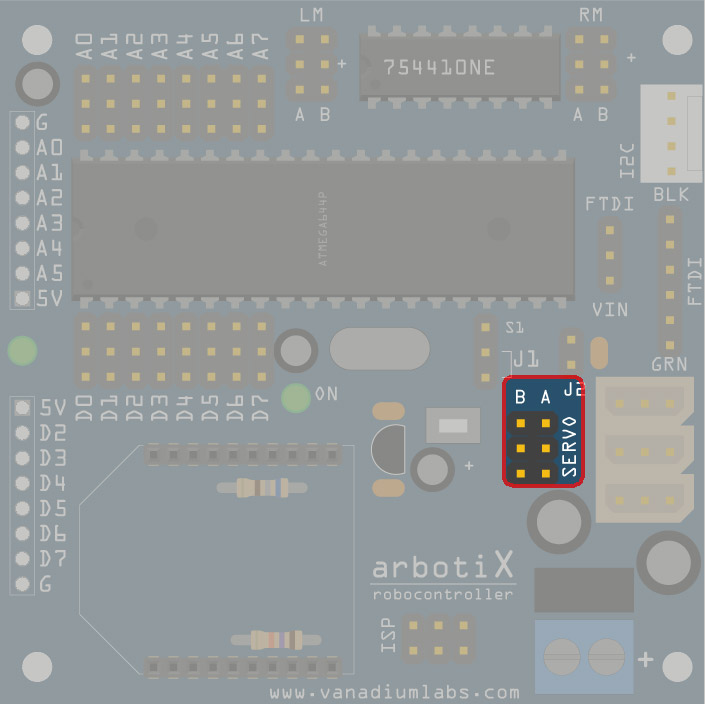
\includegraphics[scale=0.2]{imagenes/arbotix_hobby_servo.jpg}
%\caption{Ilustración de los puertos Hobby de la Arbotix}
%\label{fig:puertosHobby}
%\end{figure}

%\begin{figure}[hbtp]
%\centering
%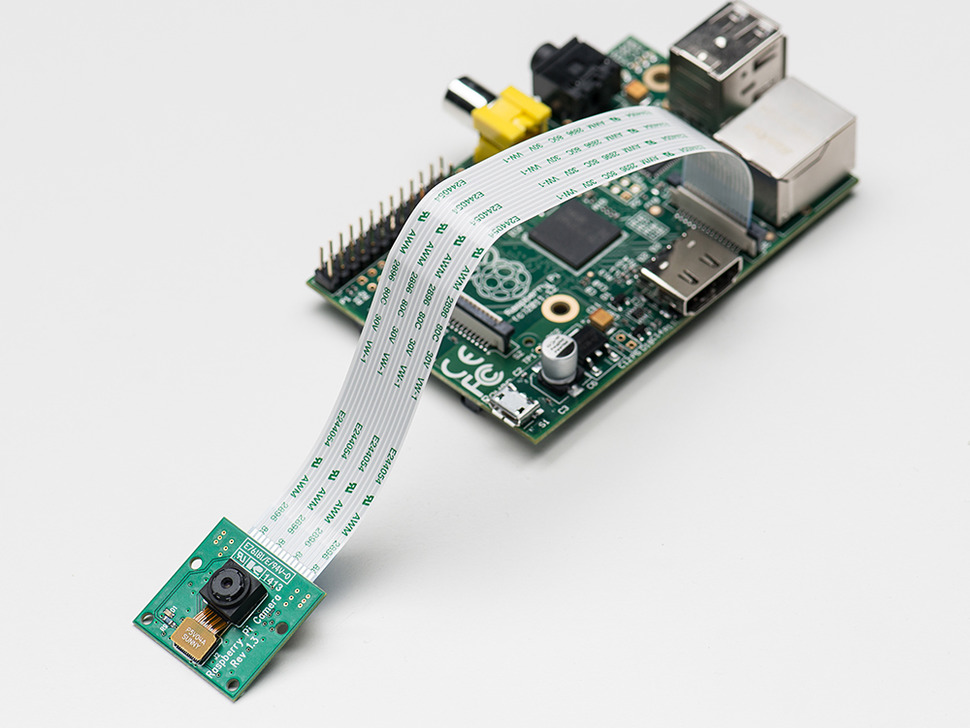
\includegraphics[scale=0.6]{imagenes/raspbCam.jpg}
%\caption{C\'amara Raspberry Pi conectada al puerto CSI de la tarjeta}
%\label{fig:camACSI}
%\end{figure}
 
\begin{figure}[hbtp]
\centering
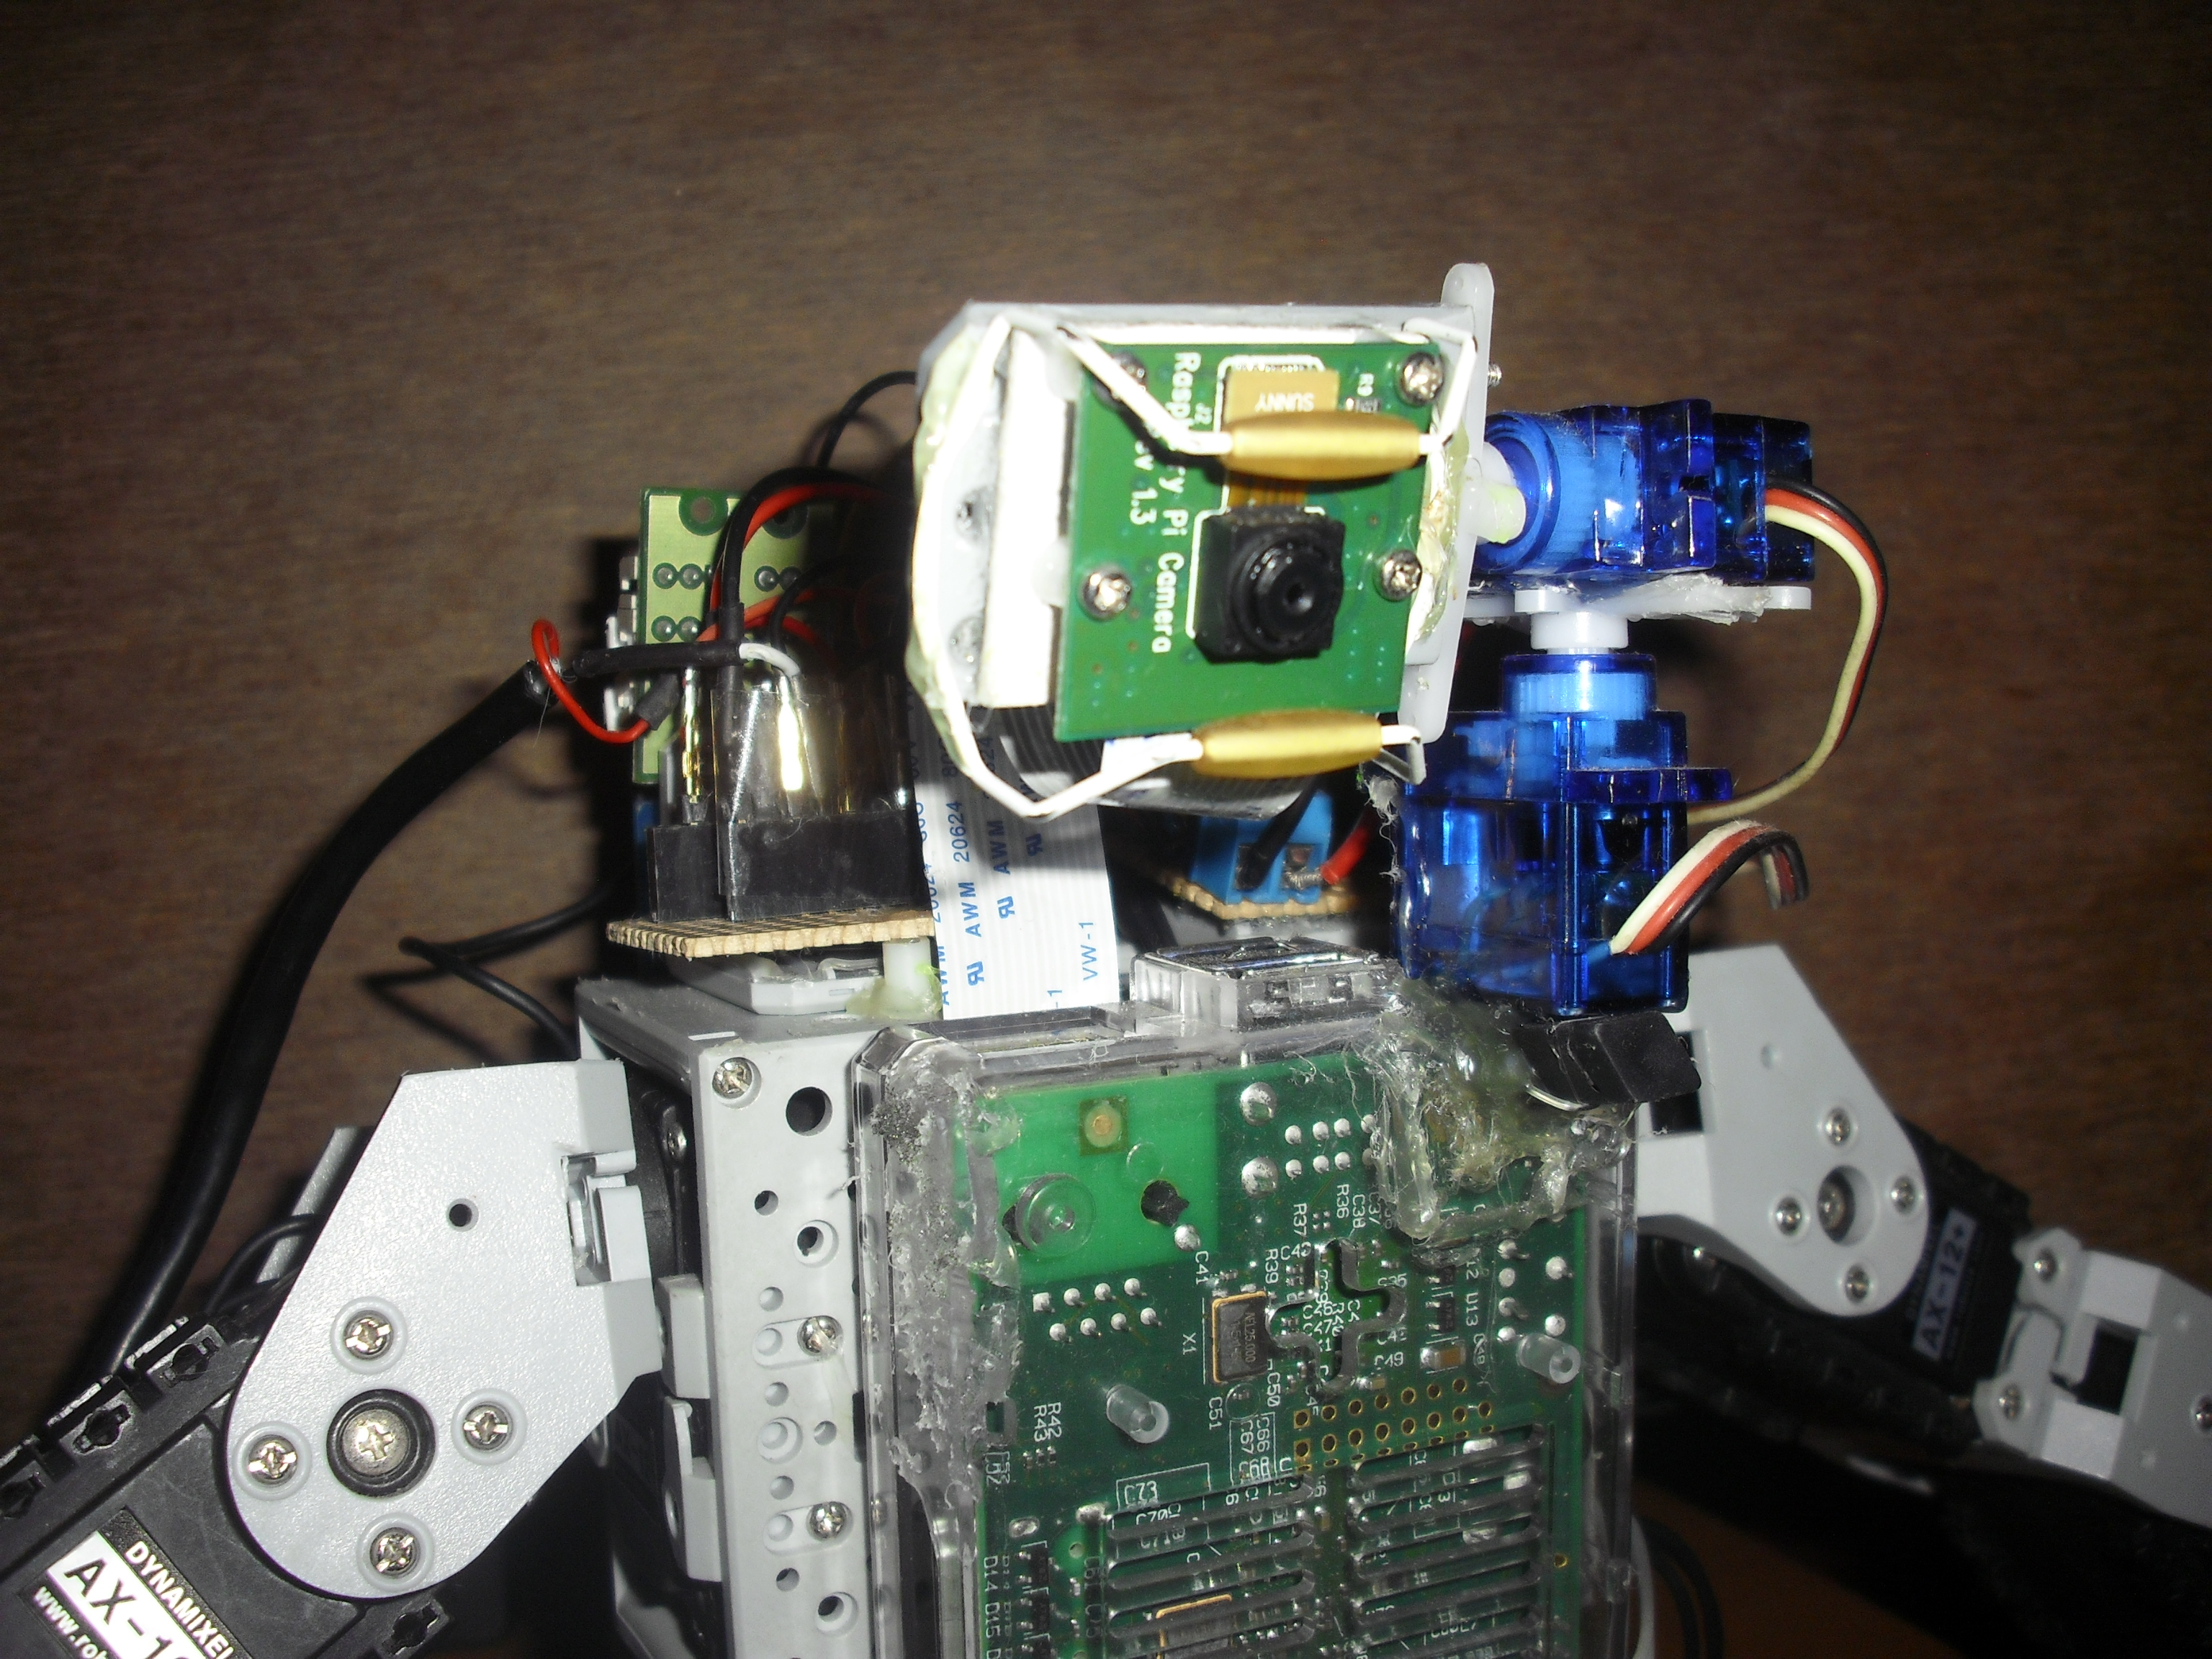
\includegraphics[scale=0.05]{imagenes/servosYcamara.JPG}
\caption{Parte delantera del robot incluye c\'amara, los dos servo motores (azules) y Raspberry Pi}
\label{fig:servosycam}
\end{figure}

Los motores Dynamixel se conectan a la controladora Arbotix por medio de los puertos Bioloid de la tarjeta. El diseño de Junny posee cuatro extremidades: dos brazos y dos piernas, por lo que naturalmente, el conjunto de motores, se puede descomponer en cuatro cadenas o series separadas. Sin embargo la Arbotix s\'olo cuenta con tres puertos Bioloid. Se consideró la opción de unir dos extremidades pero ello implicaba limitaciones en el movimiento del robot, por lo tanto se optó por agregar un expansor de puertos Bioloid y así conectar cada extremidad en un puerto diferente. La forma en la que se ha conectado estos motores se ejemplifica en la figura ~\ref{fig:arbotixConectados}. 

\begin{figure}[hbtp]
\centering
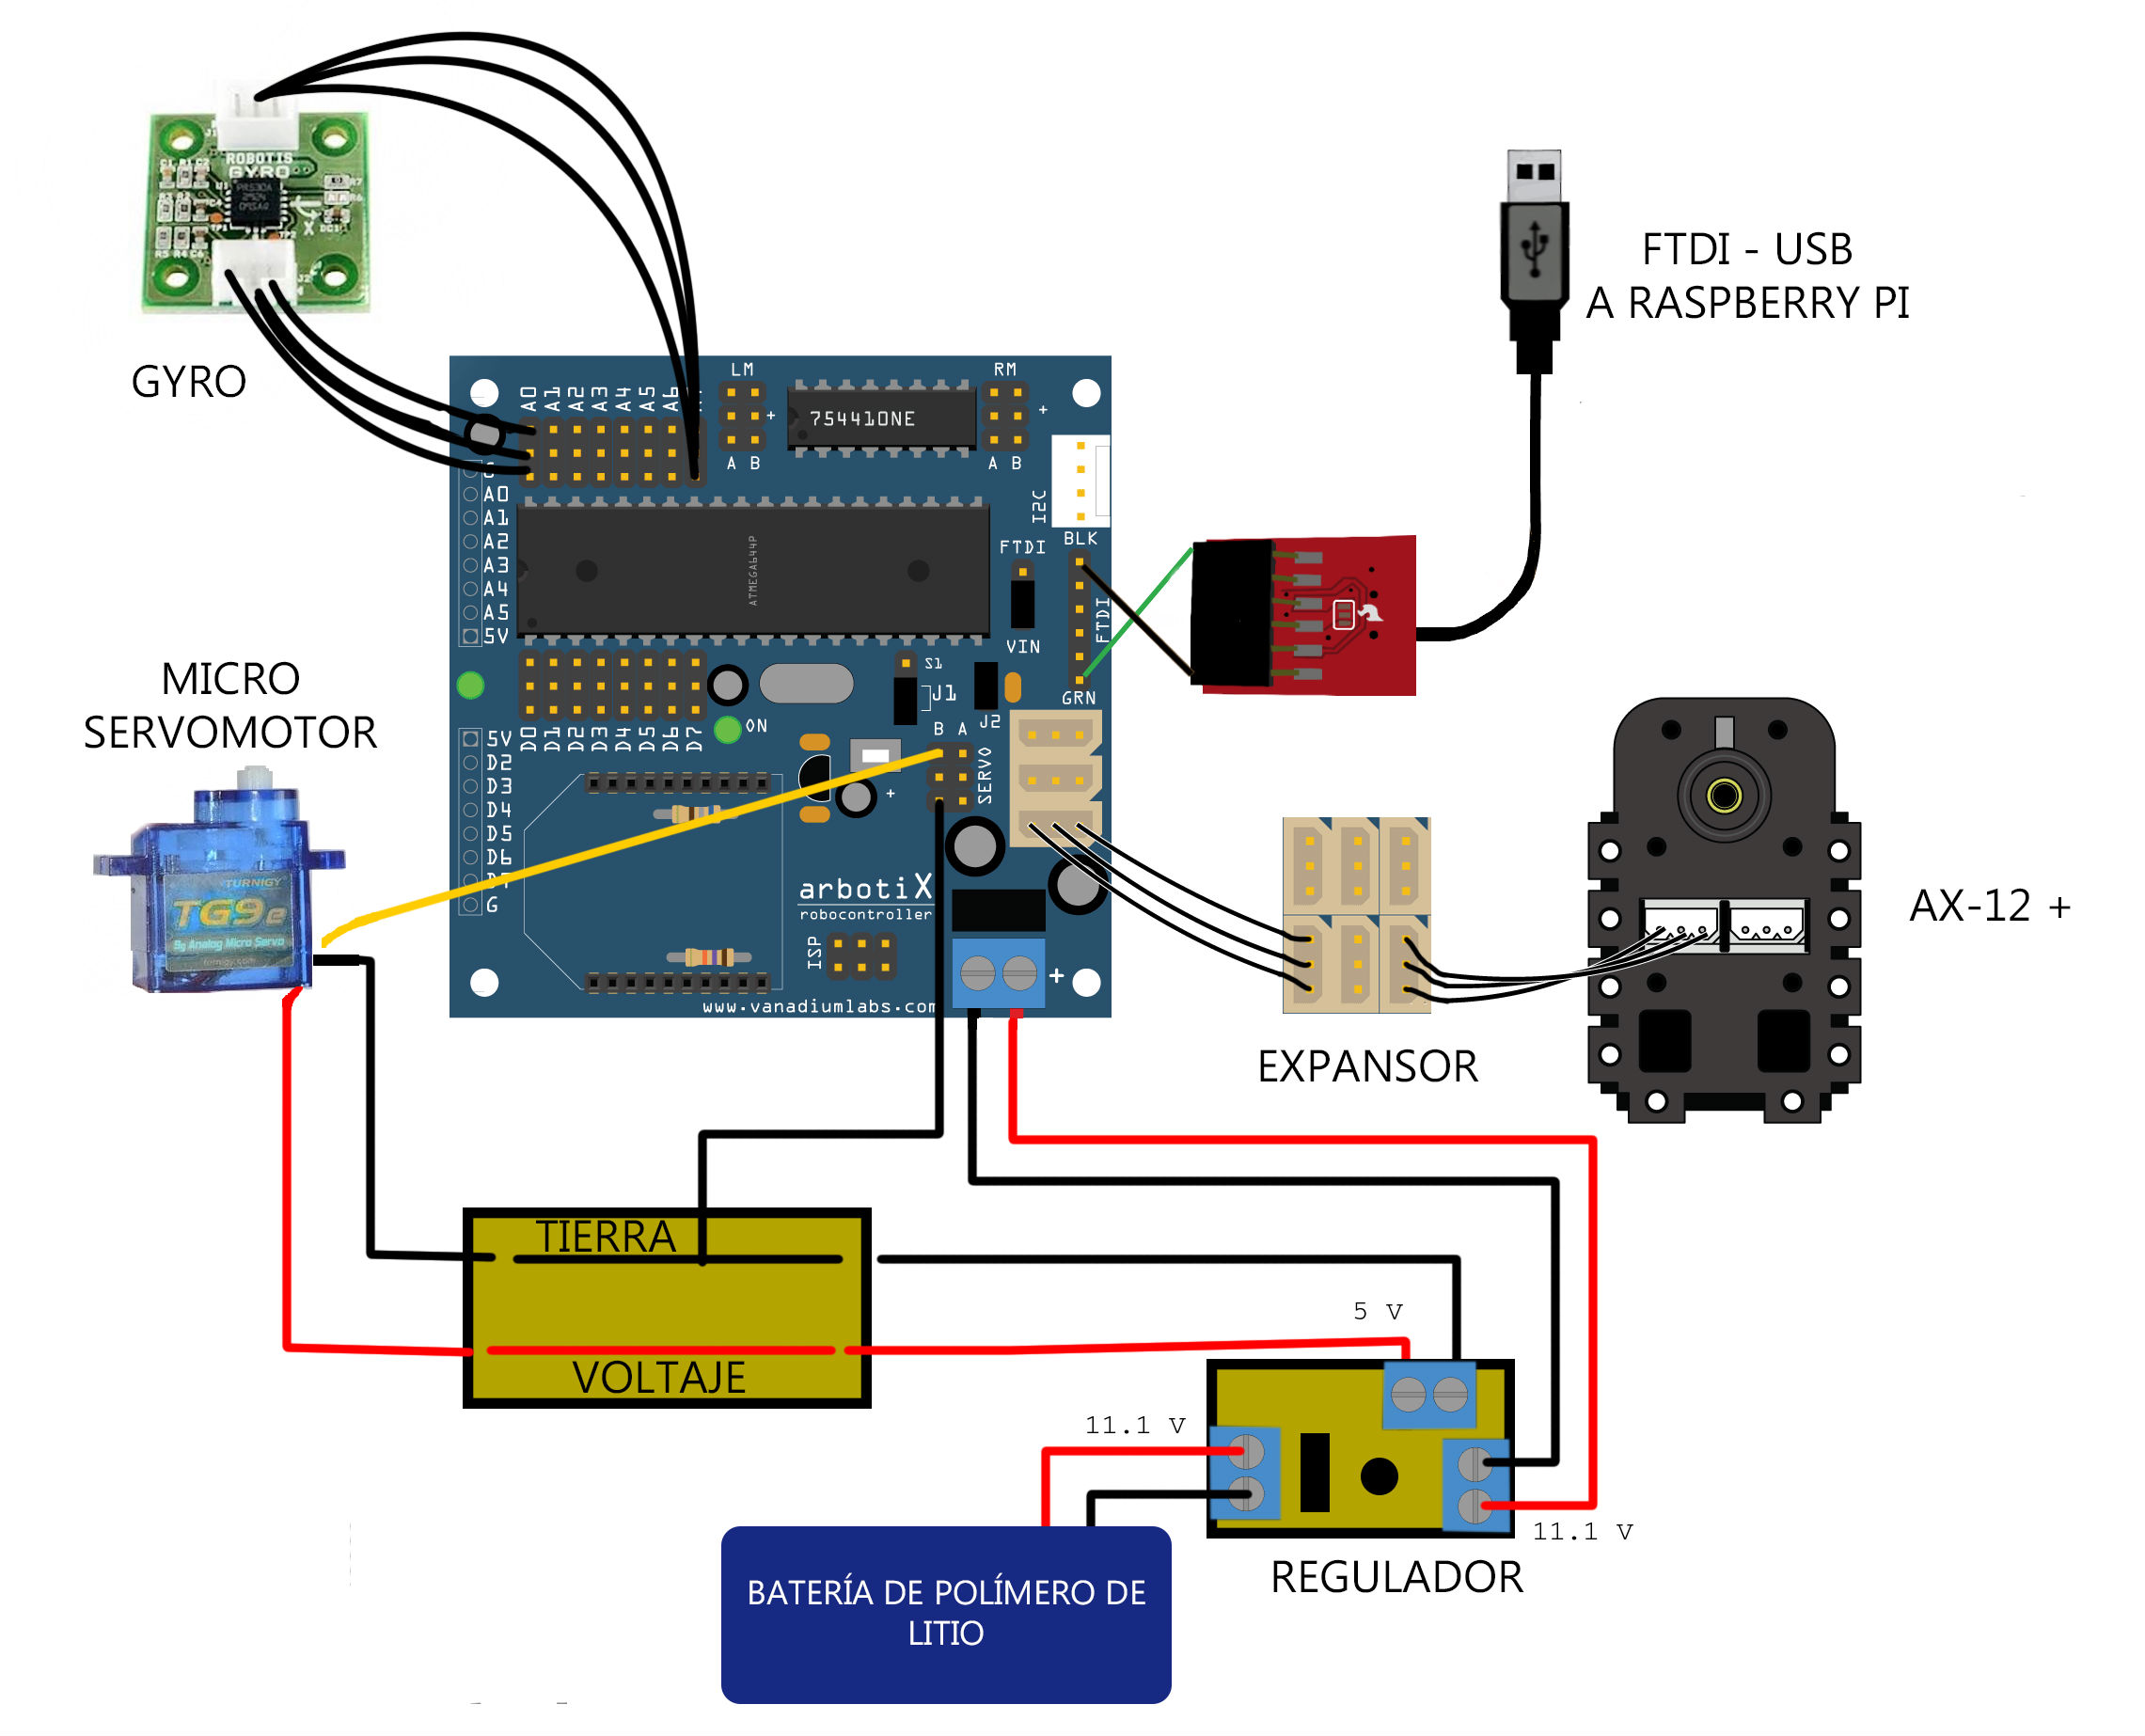
\includegraphics[scale=0.2]{imagenes/arbotix_componentes1.jpg}
\caption{Tarjeta controladora Arbotix y componentes conectados (Imagen referencial: el regulador se encuentra dispuesto en diferente orden)}
\label{fig:arbotixConectados}
\end{figure}

La comunicación de la tarjeta de Arbotix con la computadora, incluso con la Raspberry Pi, se realiza a través del chip FTDI, un extremo se conecta en el puerto FTDI de la tarjata Arbotix, como lo ilustra la figura ~\ref{fig:arbotixConectados}, y el otro extremo se conecta al puerto \gls{USB} de la tarjeta Raspberry Pi.

Para evitar agregar peso innecesario al robot se decidi\'o usar una sola fuente de poder. Se utilizó una batería de polímero de litio de 11.1 V y 1 A. Y se construyó un circuito para regular el voltaje de los componentes que necesitan 5 V (ver figura ~\ref{fig:circuito}).



